\chapter{Advanced ToM+ configurations}

\section{The WiFi settings page}
\label{sec:wifi_settings}

Since the second firmware release, your ToM+ can now connect to the Internet by a Wi-Fi
on board module. This will allow you to view your Twizy real time data if combined
with MQTT protocol which will be dealt in Section~\ref{sec:MQTT}.\\

\begin{figure}[H]
    \centering
    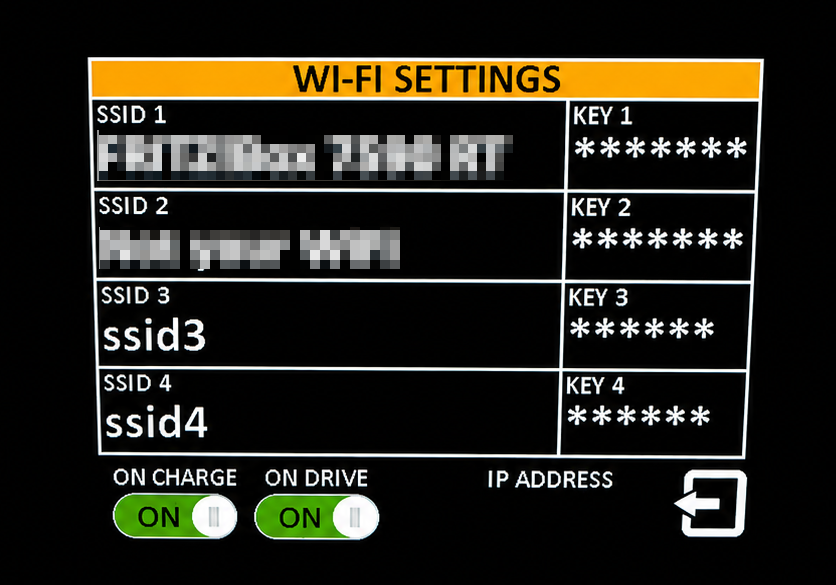
\includegraphics[width=0.8\textwidth]{figures/wifi_settings_3d.png}
    \caption{The WiFi settings page.}
\end{figure}

The page will store up to four connection profiles in order to be connected to the
Internet when you are at home or even at work or in a public place with a free Wi-Fi.
\\In addition ToM+ has a web interface, in which you can monitor data in real time
or customize your settings much more easily. Now let's see why you should do this…

\subsection{ToM+ WiFi advantages}

Since the second firmware release, your ToM+ can now connect to the Internet by a Wi-Fi
embedded module and this will allow you to unlock many more features than before.
Now you can have access to your Twizy data remotely on your smartphone!\\

You won't need to manually check your Twizy charging state anymore, because this
new feature will publish charging state data directly on your smartphone and they
will be protected and private as well. It will just need some MQTT configuration.\\

\begin{itemize}
    \item No more struggling on constantly checking your Twizy charging state manually!
    \item Plenty of possibilities to embed your Twizy in an IoT system relying on MQTT
    \item Wi-Fi would not affect much both electric consumption and ToM performances 
    \item Unlock a new web page with real time Twizy data and ToM user-friendly settings
\end{itemize}

\subsection{Adding a WiFi connection profile}
\label{sec:add_wifi_profile}

In this new settings page you have a small table with four rows and two columns.
The first column holds the \textbf{SSID} (i.e. the name) of the network you are trying to connect to. 
To be clear it's the one you see on your phone or laptop. It can be alphanumeric and 
it is case sensitive (capital letters matter, so be sure to spell it correctly!).
While the second column under the \textbf{“KEY”} header is for the Wi-Fi password.\\

When you tap on a table cell, either SSID or key, ToM+ will open a keyboard page
where you can type in your data. Pressing OK will confirm the typed string and will
take you back to the Wi-Fi settings page. We will discuss the keyboard page in Section~\ref{sec:keyboard_page}.\\

By now you are able to set \textbf{four different connection profiles} with four pairs of SSID
and password. If you don't set any profile but the Wi-Fi slider are enabled ToM+ will still
perform a Wi-Fi scan every two minutes trying to find public connection without password
protection and then it will try to connect. Press the bottom \textbf{right arrow button to save}.

\subsection{Check WiFi connection}
\label{sec:check_wifi_connection}

To check if your ToM+ is connected to the Internet via Wi-Fi the process is very
simple. In all pages there is the WiFi icon (dealt in Section~\ref{sec:status_icon_bar})
which shows its status.

\iconbox{icons/Tray_WiFiOff.png}
{WiFi is off}
{ToM+ is not connected and won't publish any data.}

\iconbox{icons/Tray_WiFi.png}
{WiFi is on}
{ToM+ is connected and will publish data if MQTT is connected.}

\iconbox{icons/Tray_WiFi.png}
{WiFi scan in progress}
{If blinking, ToM+ is currently scanning for available Wi-Fi networks.}

\clearpage

If you want to get more specific info about whether or not your ToM+ is connected to
any network, you can check additional fields in the Wi-Fi settings page on the bottom right
corner, as shown in the image below.

\begin{figure}[H]
    \centering
    
\includegraphics[width=0.7\textwidth]{figures/wifi_bottom_line.png}
    \caption{The WiFi bottom grid info.}
    \label{fig:wifi_bottom_line}
\end{figure}

As we can see when the ToM+ is connected to a network an IP address will be
displayed (here it is \textbf{10.24.126.204}). This is the address taken by ToM+ to connect
to the Internet. If this field contains any sequence of four numbers (from 0 to 255)
separated by dots, then Wi-Fi is connected, otherwise it will be empty. 

Tap on it to view ToM+ MAC address and tap again to see which SSID (network name) ToM+ is connected to.
We will see more interesting features in which ToM+ IP address is involved later at Section~\ref{sec:access_webserver}.

\subsection{Enable/Disable WiFi features}
\label{sec:enable_disable_wifi}

In the footer of the Wi-Fi settings page there are two sliding buttons. To change from
ON and OFF state just tap or slide it. Let's see what the two sliders do.\\

The first one of them is to disable \textbf{Wi-Fi when charging}. This will cause your ToM+ to be completely offline,
and you won't be able to monitor your Twizy data remotely until you enable it again.
In this state the Wi-Fi status icon will be always grayed out as shown in Section~\ref{sec:check_wifi_connection}.\\

The second sliding button is to enable \textbf{Wi-Fi when driving}. This will allow
your ToM+ to be connected to the Internet even when you are driving your Twizy.
This is useful if you want to publish real-time data to your smartphone via MQTT.
This also enables the web interface to be accessed while driving and your ToM+ will
scan for available Wi-Fi networks as well.\\

As already mentioned to \textit{save your changes} you need to press the bottom right arrow button.
If you don't do this, your changes will be lost when you leave the page.

\clearpage

\section{The MQTT settings page}
\label{sec:MQTT}

If you have already took a look at the Wi-Fi Section~\ref{sec:wifi_settings}, you would probably now
know that MQTT is needed to access to your data remotely and this section will show
you how to set up it correctly and how does the ToM+ interface deal with this protocol.

\begin{figure}[H]
    \centering
    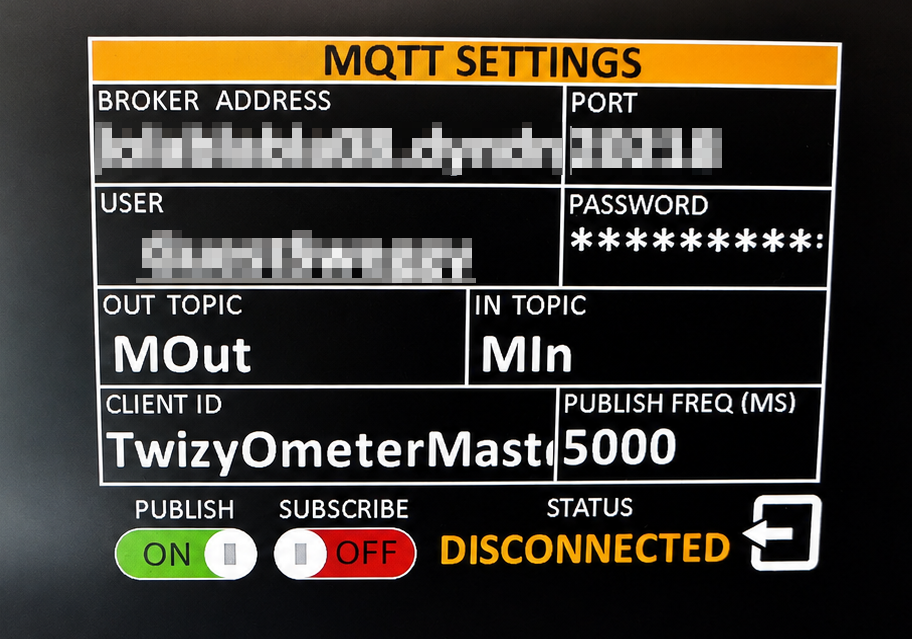
\includegraphics[width=0.8\textwidth]{figures/mqtt_settings_page.png}
    \caption{The MQTT settings page.}
\end{figure}

When ToM+ is connected to the Internet via Wi-Fi, MQTT can be enabled and then
you can view your real time Twizy data directly on your devices. The page only
allows only one MQTT server configuration, to ensure \textbf{data safety and privacy}. You
can configure this parameters both on ToM+ and on its Web Server page (Section~\ref{sec:web_network_settings}).
Now let's discuss what's MQTT and some of its main advantages…

\subsection{Brief MQTT explanation}
\label{sec:brief_mqtt}

MQTT is one of the easiest protocols used in IT to communicate small data payloads
using a \textbf{client/server architecture}. This method requires one or more clients that
usually collect data and want to store them permanently and/or perform calculations.


So the process needs a server which processes data from all clients executing tasks.
This server is called \textbf{MQTT broker} or commonly broker and is essential in this type
of architecture. But how can clients and server communicate between themselves?\\


The communication process is based on a publish/subscribe structure. Some clients
collect and publish data and for this reason they are called \textbf{publishers} and, in the
meanwhile some others wait for those data to be sent and they're called \textbf{subscribers}.
The broker server lays in the middle and is the intermediary device on which all data
from publishers are stored and sent to subscribers. Now let's introduce topics…\\


A \textbf{topic} is a sequence of alphanumeric characters typically related to a specific
subject and it's used to store (like a container) all data related to that specific
subject. Topics are useful to keep and organize a lot of data collected from different
publishers in order not to confuse those information. So, how ToM+ uses MQTT?

\subsection{ToM+ and MQTT communications}

Now that we know what's MQTT, let's see how MQTT and ToM+ system actually works.
ToM+ is considered a publisher, because it collects and publishes Twizy updated data.
The phone application instead, will be the subscriber because it is waiting to receive
those data that the Twizy has just published. But who is in the middle? The broker server.\\

Unless you have a self-hosted broker server (as I do), or you already know one to use, I
will explain how to set up your free external broker server in Section~\ref{sec:free_broker}.


So, combining ToM+ with MQTT protocol can be very powerful and if you like home
automation and IoT systems can also unlock endless possibilities. For instance, you can
create your own subscriber that will perform actions on ToM+ published data.\\

\subsection{Setting up MQTT free broker}
\label{sec:free_broker}

\textit{Disclaimer}: Take your time while doing this process because for not expert users may
take some more minutes and be sure to \textbf{note down your configuration} parameters.\\

First of all choose your MQTT broker provider, I personally advice Maqiatto, since
it's free, intuitive and easy to use. So let's visit the official website tutorial page:
\url{https://www.maqiatto.com/examples}. Now we should see a page like the one shown here:

\begin{figure}[H]
    \centering
    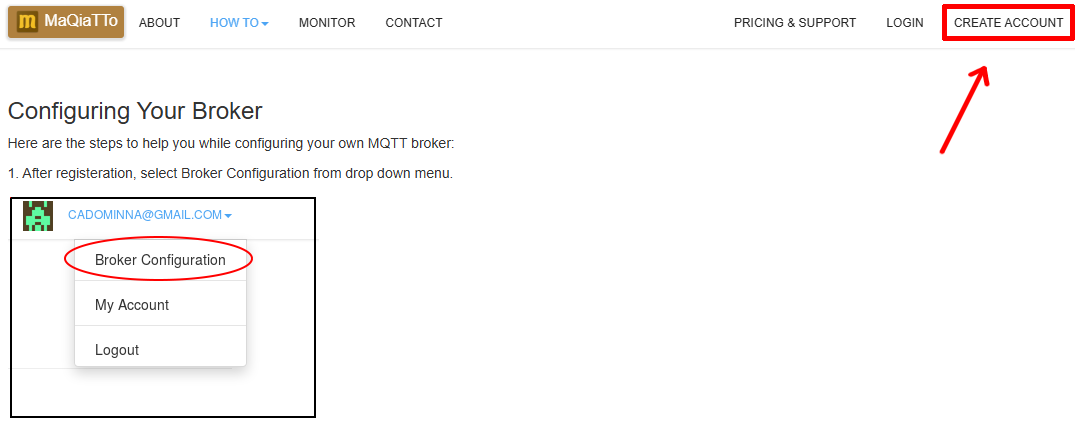
\includegraphics[width=1\textwidth]{figures/mqtt_step1.png}
    \caption{Step 1: Press “CREATE ACCOUNT” button.}
\end{figure}

As the official guide says, you need to have an account in order to create your MQTT
broker. So let's press the top right circled \textbf{“Create Account”} button and create one.
You will be redirected to this page (\url{https://www.maqiatto.com/signup}) where you will have to fill in your personal data.

\begin{figure}[H]
    \centering
    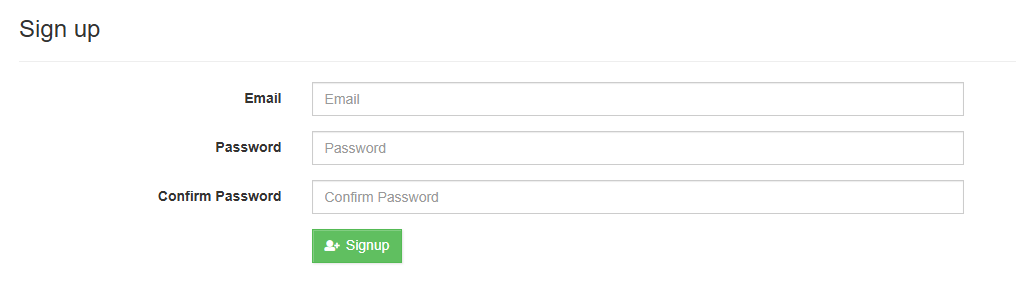
\includegraphics[width=1\textwidth]{figures/mqtt_step2.png}
    \caption{Step 2: Fill in your personal data.}
\end{figure}

After filling in all the form fields press the \textbf{“Signup”} green button and wait until we
get this page (\url{https://www.maqiatto.com/configure}) popping up a successful 
registration message as shown in the image down here:

\begin{figure}[H]
    \centering
    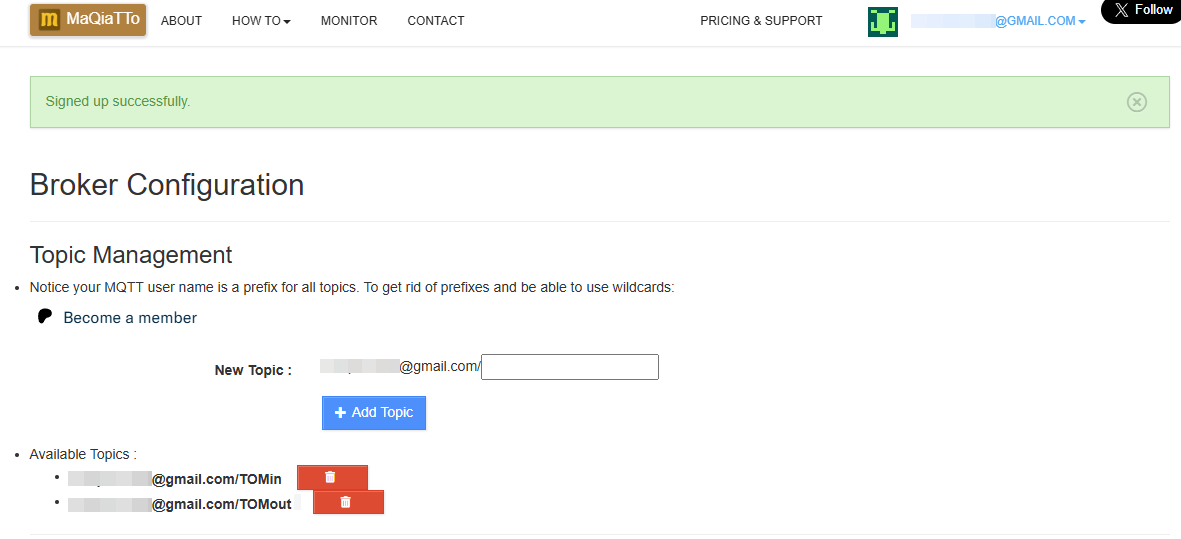
\includegraphics[width=1\textwidth]{figures/mqtt_step3.png}
    \caption{Step 3: Add IN/OUT topics.}
\end{figure}

From this page you can manage your available topics (refer to Section~\ref{sec:brief_mqtt})
and creating new ones as well. So let's create our IN and OUT topic for sending and 
receiving ToM data. As we can see, there's a fixed prefix (your email) since free
users have this limitation, but it isn't a problem at all.\\

In the blank text box after the “/” symbol we should put the name we want to give to our topics. Choose it carefully
and make sure it is clear and easy for you to remember. For instance I will call the
input topic \textbf{TOMin} and the output topic \textbf{TOMout}, but you can choose the name you
prefer.\\

For the first topic, type \textbf{TOMin} and press the \textbf{“+ Add Topic”} blue button as I did above.
If the operation ends up correctly then a green popup message will show, saying
\textbf{“Topic was added for this user”} and a new records will appear in the \textit{“Available
Topics”} list that was empty before. Now repeat the process for the \textbf{TOMout} topic as
well and check again if the topic was successfully created. Before this process the \textit{“Available
Topics”} list was empty, but now we can see our two topics in the list and we can delete them if needed.

\begin{figure}[H]
    \centering
    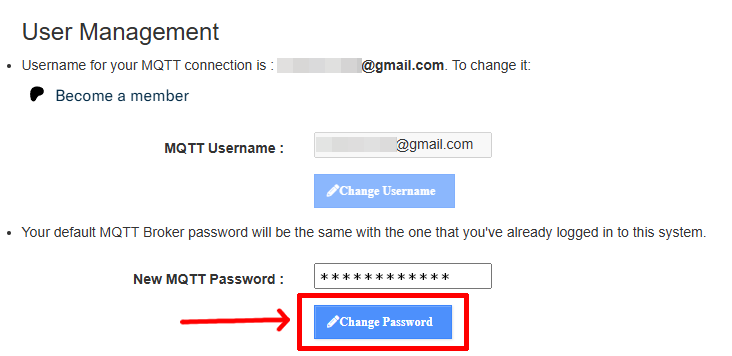
\includegraphics[width=0.8\textwidth]{figures/mqtt_step4.png}
    \caption{Step 4: Change your broker password.}
\end{figure}

\textit{This step is suggested but optional}. At this point the broker password is the same 
of your Maqiatto account and it is not secure at all. But if you don't want to 
change it or you don't care, you can skip this step and go to the next one.\\

So let's take some time to make the broker secure and protected from unwanted access.
The second part of this page (\url{https://www.maqiatto.com/configure}) allows you to change your broker password.
Just type the new one in the \textbf{“New MQTT Password”} text field and
then press the \textbf{“Change Password”} blue button.


If everything goes well, a green popup message will show up saying \textbf{“Broker user password was updated”}.
The change username button is greyed out because you can't change your username unless you are a premium user.

\begin{figure}[H]
    \centering
    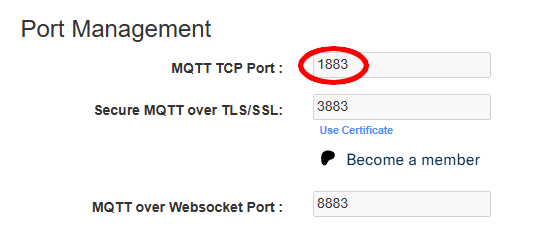
\includegraphics[width=0.7\textwidth]{figures/mqtt_step5.png}
    \caption{Step 5: Note down the port number.}
\end{figure}

In the last section of the configuration page (\url{https://www.maqiatto.com/configure})
there are the \textbf{“Port Management”} parameters. Note down the MQTT TCP Port 
which is usually set to \textbf{1883} (just to be sure) because it's the standard well-known
port number over the Internet for MQTT protocol. Now the MQTT broker is ready to be
used and we can move on to the next step, which is configuring ToM+ with the broker parameters.

\clearpage

\subsection{Connect ToM+ to MQTT broker}

Now that it's clear what MQTT (Section~\ref{sec:brief_mqtt}) is and we have set up our
personal broker (Section~\ref{sec:free_broker}) let's see where on the display we can
connect ToM+ with our freshly created broker.

\begin{figure}[H]
    \centering
    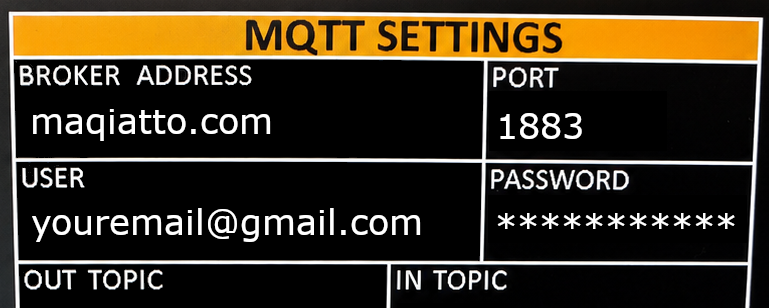
\includegraphics[width=0.8\textwidth]{figures/mqtt_connect1.png}
    \caption{MQTT broker connection parameters.}
\end{figure}


When you tap on the respective table field, ToM+ will open a keyboard page where you can type your data, as in Wi-Fi settings.
To insert the symbols or numbers press the \textbf{“1/3”} button on the keyboard to switch charset.
By pressing \textbf{OK}, you will confirm the typed string and will take you back to the MQTT
settings page. To know more about the keyboard page see Section~\ref{sec:keyboard_page}.
If the value is too long for the field, the text would automatically scroll.\\

The first thing to specify is your \textbf{broker address}. In the example shown,
it's set to \textit{“maqiatto.com”}. This is the address of the broker server that we have just created in Section~\ref{sec:free_broker}.

Then it's time to specify the \textbf{port number} where the MQTT service is running. Unless
you have set it to a different number manually the MQTT port will always be \textit{1883}.

Next we have the \textbf{user} field, which is the username that ToM+ will use to authenticate
when connecting to the broker. Since the pair of username and password is unique to
you, this will prevent unwanted user to have access to your private broker. In your case,
the user is your Maqiatto account e-mail, written like \textit{youremail@example.com}.

Afterwards we need to specify the \textbf{password of the broker} which can be different from
the one of your Maqiatto account if you chose to change it when suggested in Section~\ref{sec:free_broker}. 

\begin{figure}[H]
    \centering
    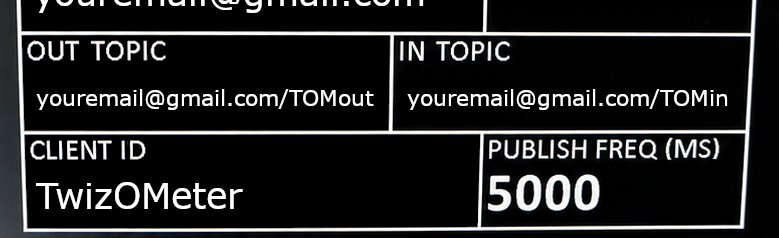
\includegraphics[width=0.8\textwidth]{figures/mqtt_connect2.png}
    \caption{MQTT ToM+ publishing parameters.}
\end{figure}


Now let's configure our \textbf{OUT topic}, where ToM+ will publish Twizy data. In Section~\ref{sec:free_broker}
we created an out topic called TOMout but the full name of the topic must include 
also \textbf{your e-mail as a prefix} followed by a “/” symbol and the topic
name “TOMout”. In the example it is set to \textit{“youremail@gmail.com/TOMout”}.

Now it's time for the \textbf{IN topic}, where ToM+ will receive MQTT commands.
As for the OUT topic, we created an in topic called TOMin but the full name
of the topic must include also \textbf{your e-mail as a prefix} followed by a “/”
symbol and the topic name “TOMin”. In the example it is set to \textit{“youremail@gmail.com/TOMin”}.

When an MQTT publisher sends a message to the broker its
connection is authenticated by username and password but it publishes using an alias
which \textit{you can arbitrarily choose}. It's important not to include spaces in the \textbf{Client ID},
only alphanumeric characters and symbols are allowed. Remember that it's
advisable to make it simple and clear as it is in the example: \textit{“TwizOMeter”}. 

The last parameter is the \textbf{publish frequency}, which represents the time
between each ToM+ publish. It's expressed in milliseconds \textit{(ms)} and can be
set to an arbitrarily value greater than 1000ms (one second). The default is \textit{5000 ms}
(five seconds) and it is a good compromise between data freshness and network usage.\\

To \textbf{save your changes} you need to press the bottom right arrow button. If you don't
do this, your changes will be lost when you leave the page. Now ToM+ is ready to 
publish and receive data via MQTT protocol.\\

\subsection{Enable/Disable MQTT features}
\label{sec:enable_disable_mqtt}

If you want to temporarily or permanently disable the publishing of data with MQTT
protocol press or slide on the left slider called \textbf{“PUBLISH”} in the image down
here. From then on ToM+ won't publish Twizy data via MQTT until you enable it again.

\begin{figure}[H]
    \centering
    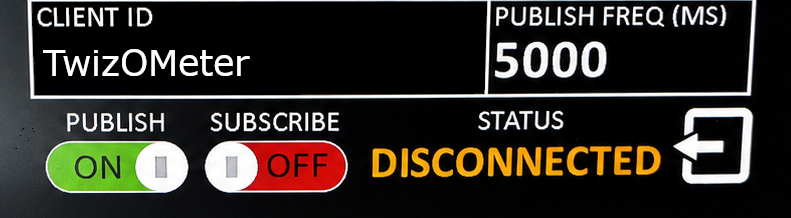
\includegraphics[width=0.8\textwidth]{figures/mqtt_connect3.png}
    \caption{MQTT bottom sliders.}
\end{figure}

The right slider button under \textbf{“SUBSCRIBE”} allows ToM+ to receive commands
from external devices published on the specified IN topic. This is useful if you
want to control via MQTT a device connected to ToM+ expansion port
(e.g. a smart plug to turn on/off charging remotely). You can choose to enable or disable this feature at any time by pressing or sliding the button.\\

\subsection{Check ToM+ MQTTconnection}

Near the two sliding buttons, there's a small \textbf{“STATUS”} label which holds
wheter the MQTT connection is working or not. When ToM+ is connected to the MQTT
specified broker, you will see a \textit{“CONNECTED”} text. When there's a problem with
the broker connection or Wi-Fi is disabled, as we saw in Section~\ref{sec:enable_disable_wifi}, MQTT won't work
properly and a \textit{“DISCONNECTED”} message appears as in the image below.

\begin{figure}[H]
    \centering
    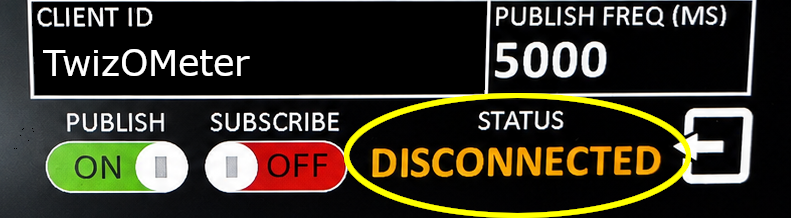
\includegraphics[width=0.8\textwidth]{figures/mqtt_status.png}
    \caption{MQTT status field.}
\end{figure}

By the way you can check the MQTT connection status also by looking at the status icon bar (Section~\ref{sec:status_icon_bar})
where the MQTT icon will be purple if the connection is established, otherwise it will be grayed.

To \textbf{save your changes} you need to press the bottom right arrow button. If you don't
do this, your changes will be lost when you leave the page.\\


\section{The Keyboard page}
\label{sec:keyboard_page}

When you tap on a table cell in the Wi-Fi or MQTT settings page, ToM+ will open a keyboard page
where you can type in your data. The keyboard page is very intuitive and easy to use.
You can switch between three different charsets by pressing the \textbf{“1/3”} button
on the bottom left corner of the keyboard.

\begin{figure}[ht]
    \centering

    \begin{subfigure}[t]{0.48\textwidth}
        \centering
        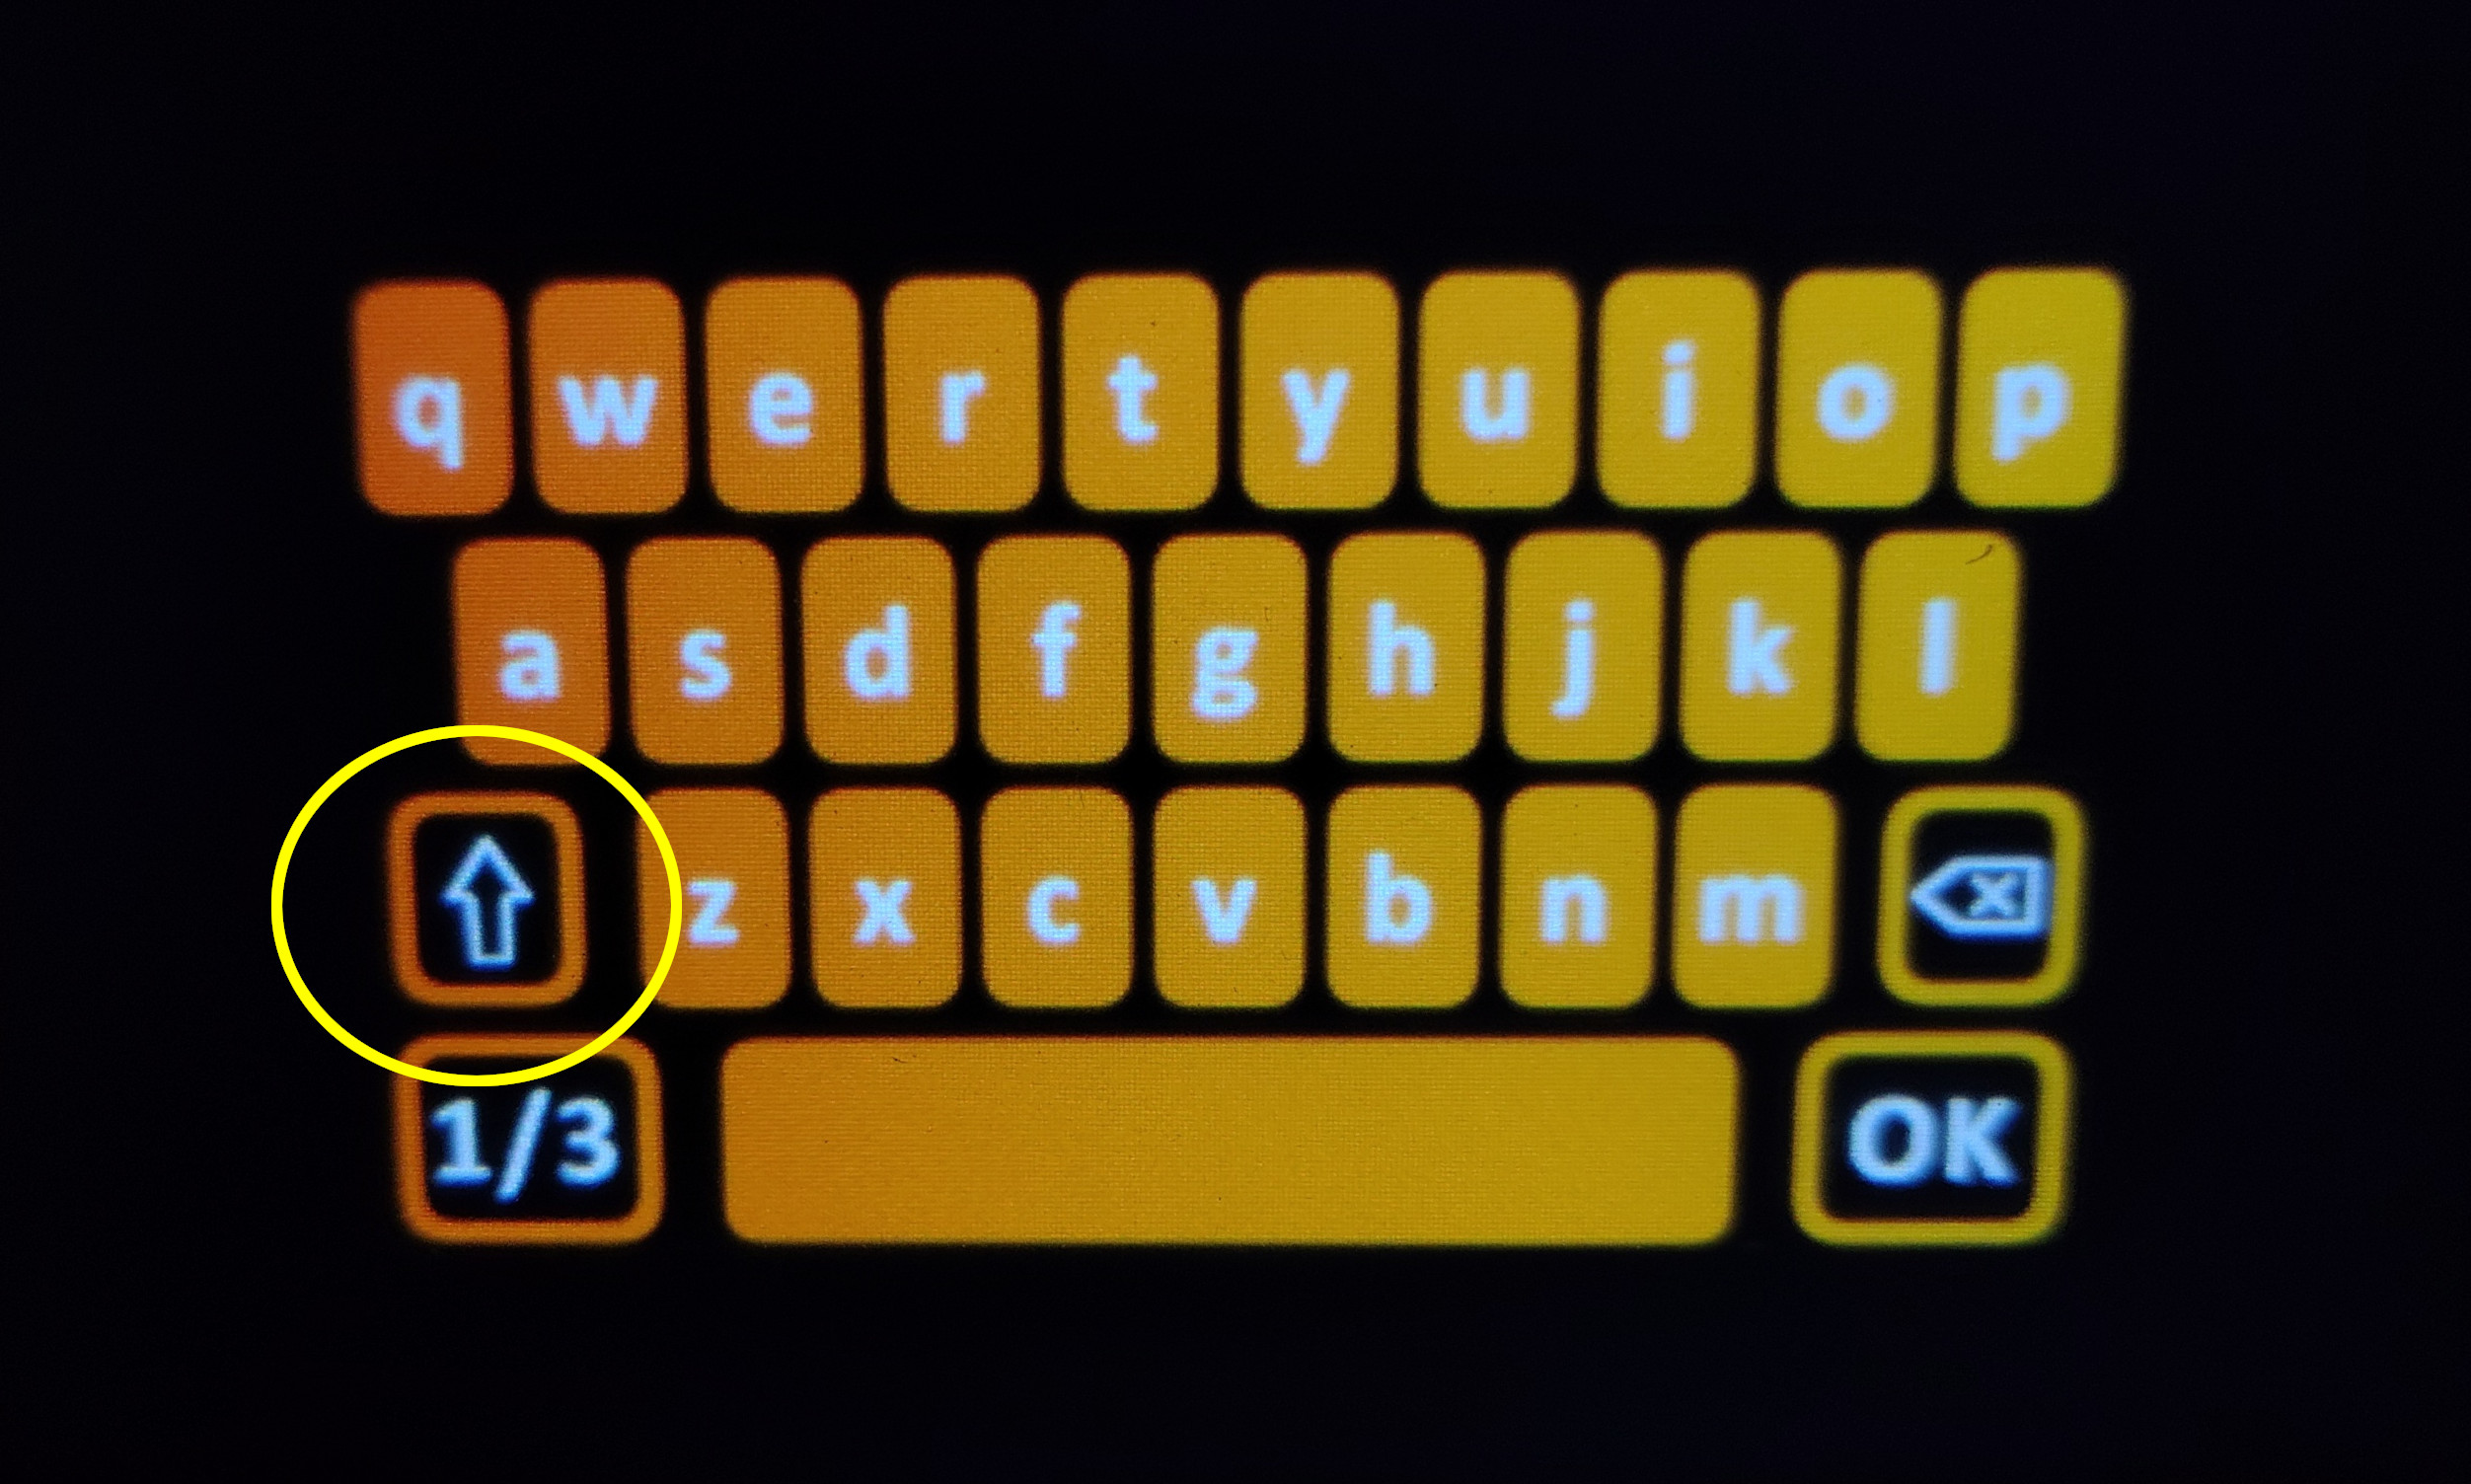
\includegraphics[width=\linewidth]{figures/keyboard_page1.jpg}
        \caption{First charset: Letters.}
    \end{subfigure}
    \hfill
    \begin{subfigure}[t]{0.48\textwidth}
        \centering
        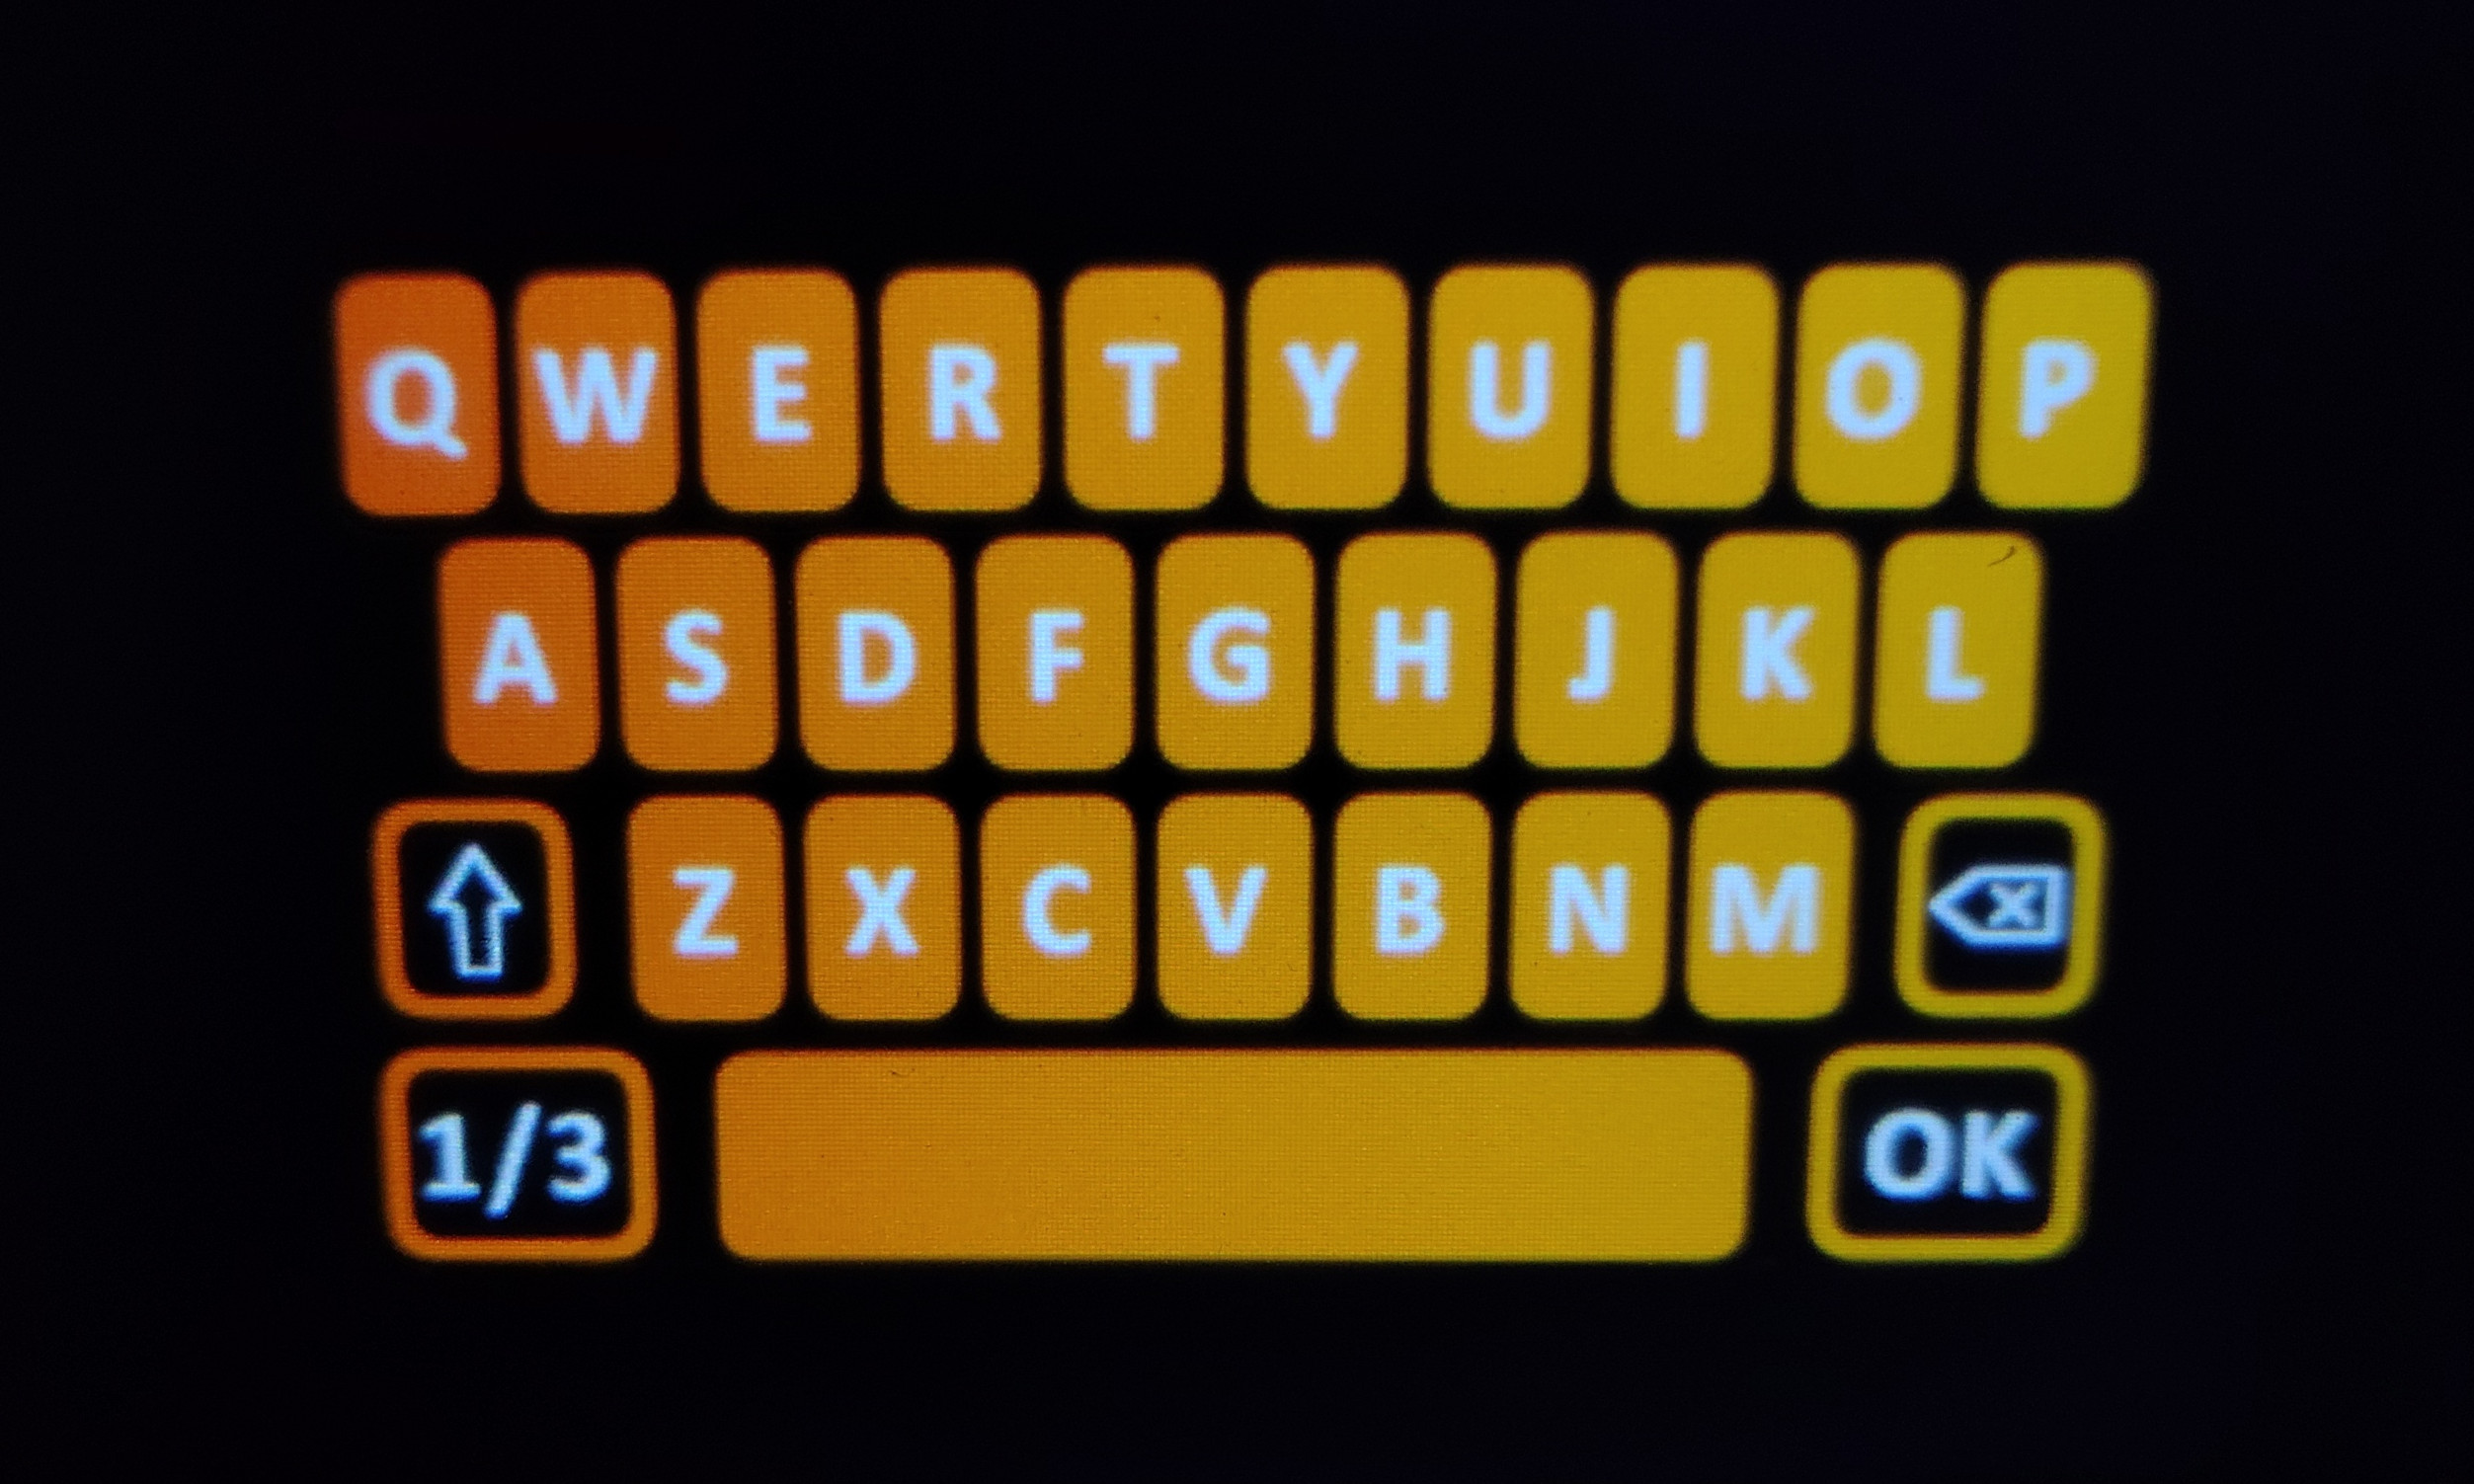
\includegraphics[width=\linewidth]{figures/keyboard_page1_caps.jpg}
        \caption{First charset: Uppercase letters.}
    \end{subfigure}
\end{figure}

In the \textbf{first charset}, you can type letters in lowercase or uppercase by pressing
the shift button circled in yellow in the first image.
When you type something it will appear in the text field on the top of the keyboard. 
If you want to delete a character just press the backspace button.

\clearpage

\begin{figure}[ht]
    \centering

    \begin{subfigure}[t]{0.48\textwidth}
        \centering
        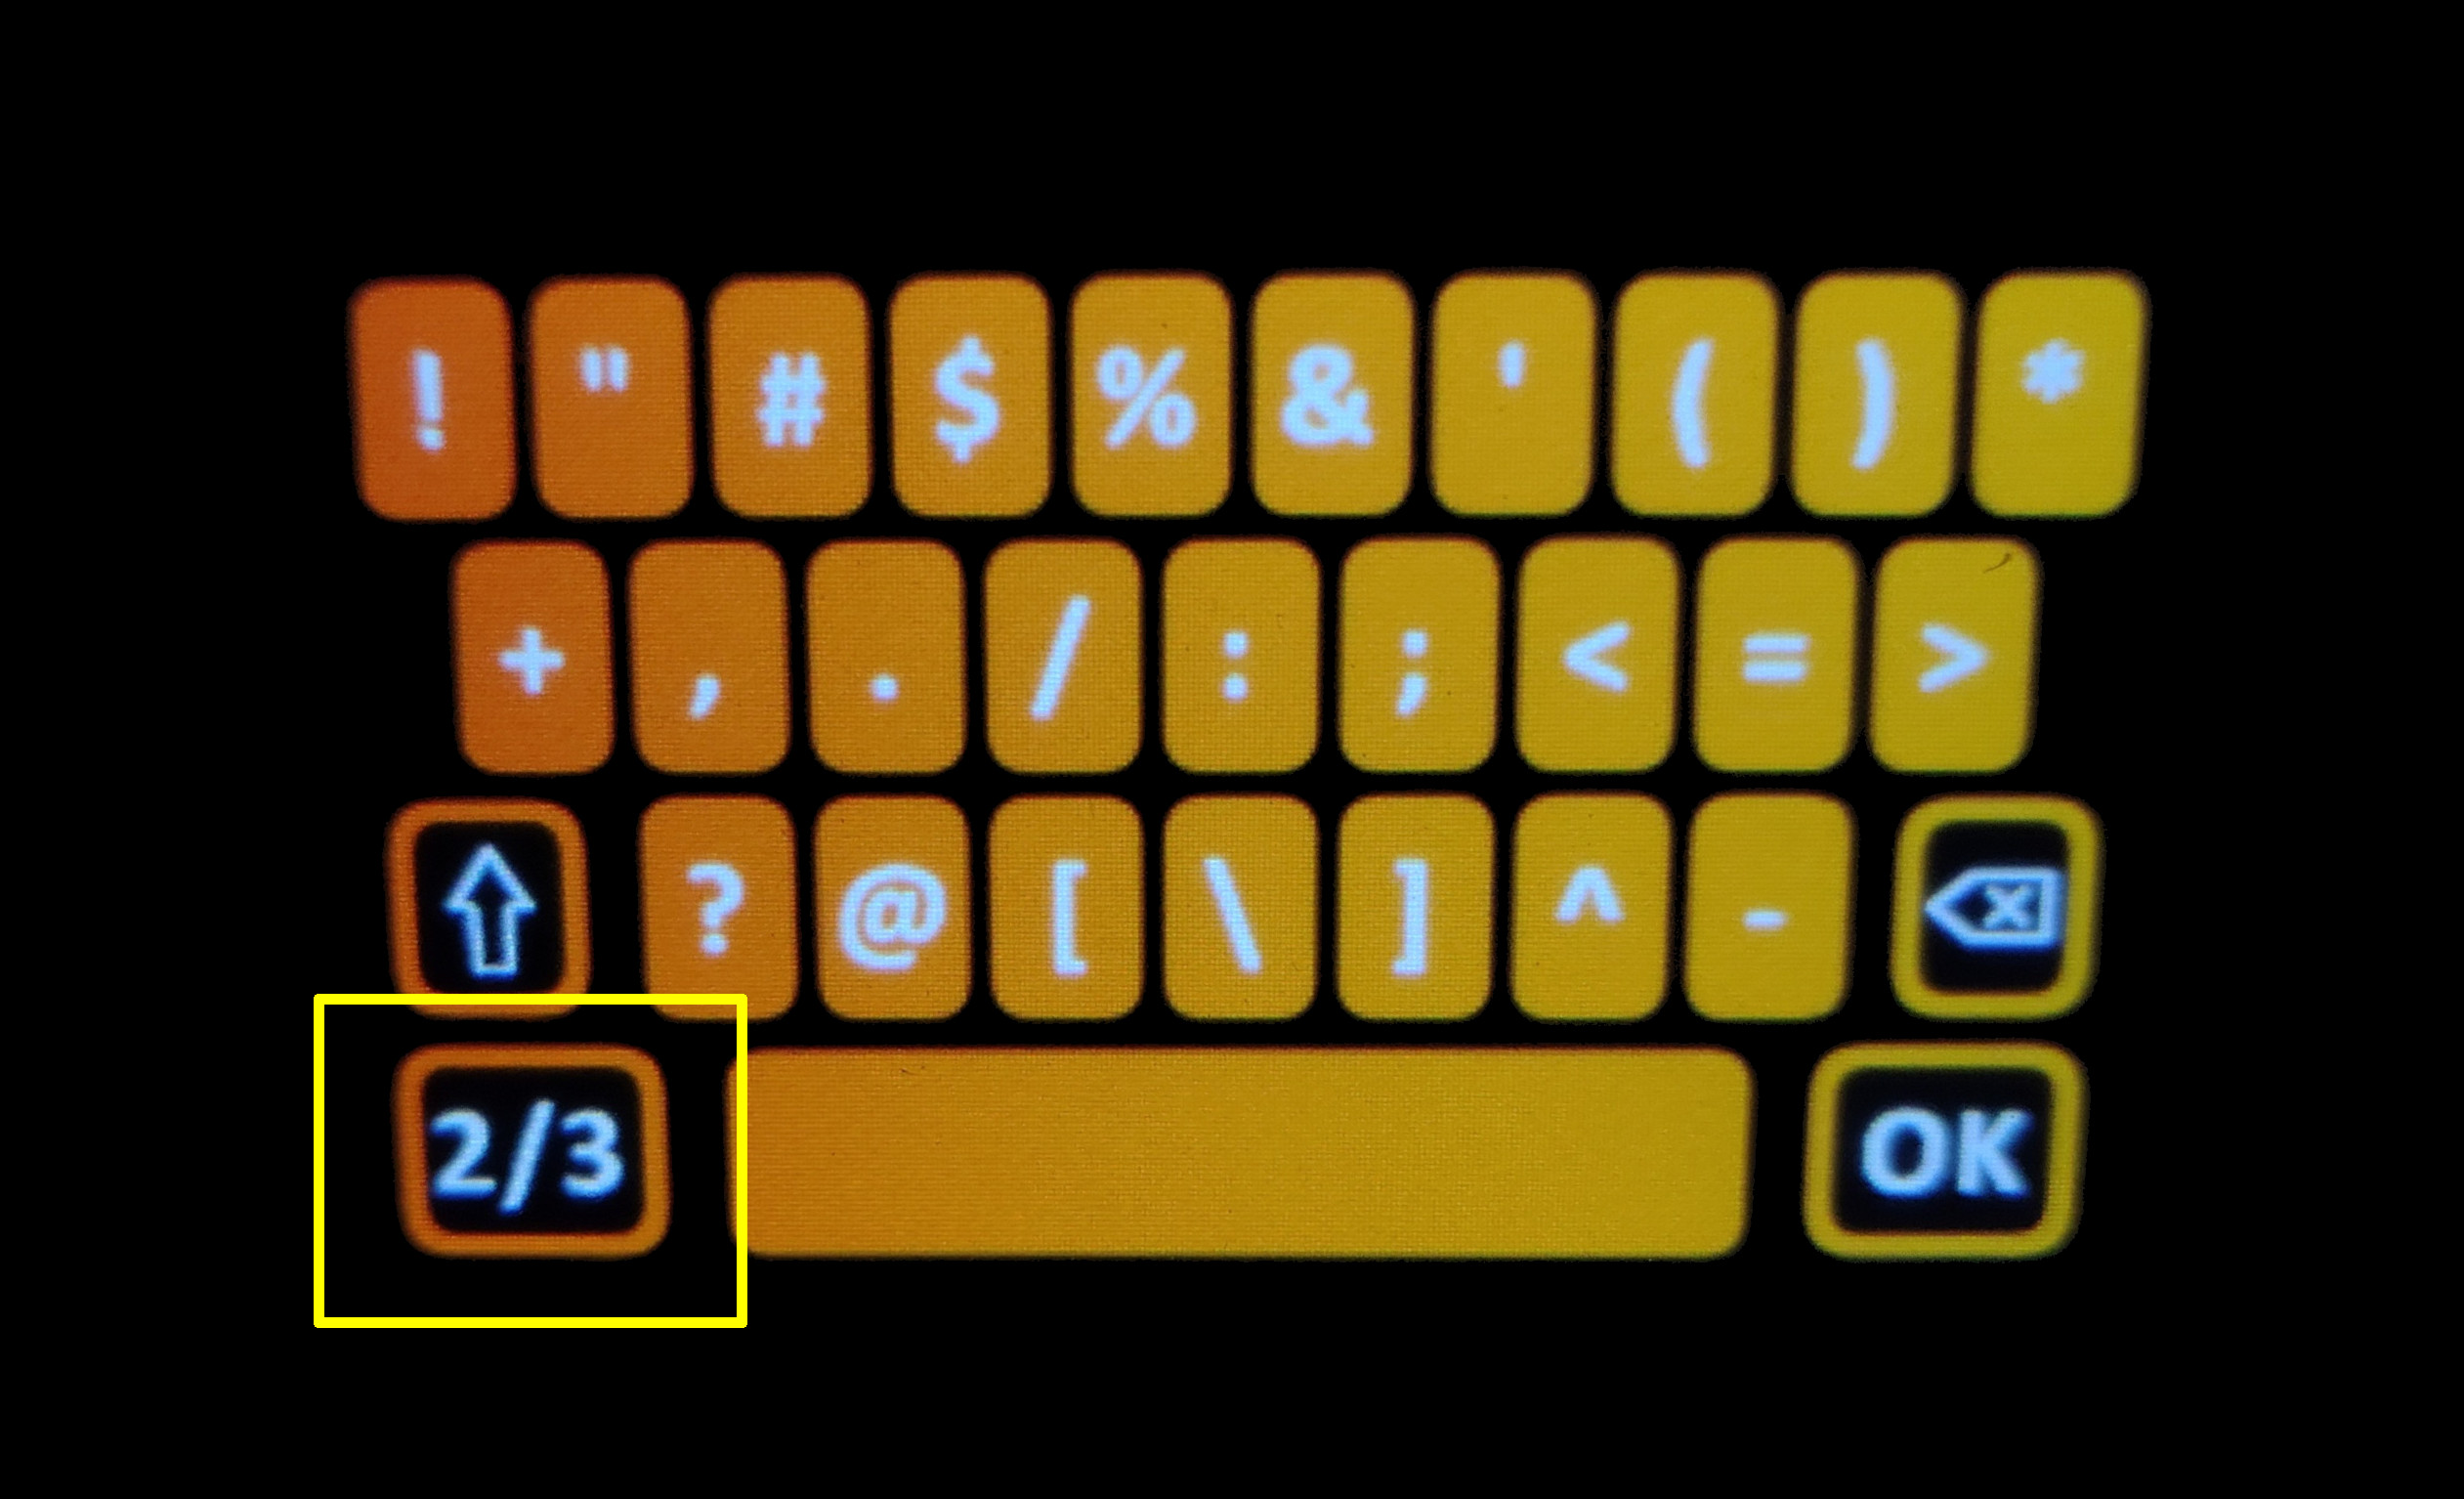
\includegraphics[width=\linewidth]{figures/keyboard_page2.jpg}
        \caption{Second charset: Symbols.}
    \end{subfigure}
    \hfill
    \begin{subfigure}[t]{0.48\textwidth}
        \centering
        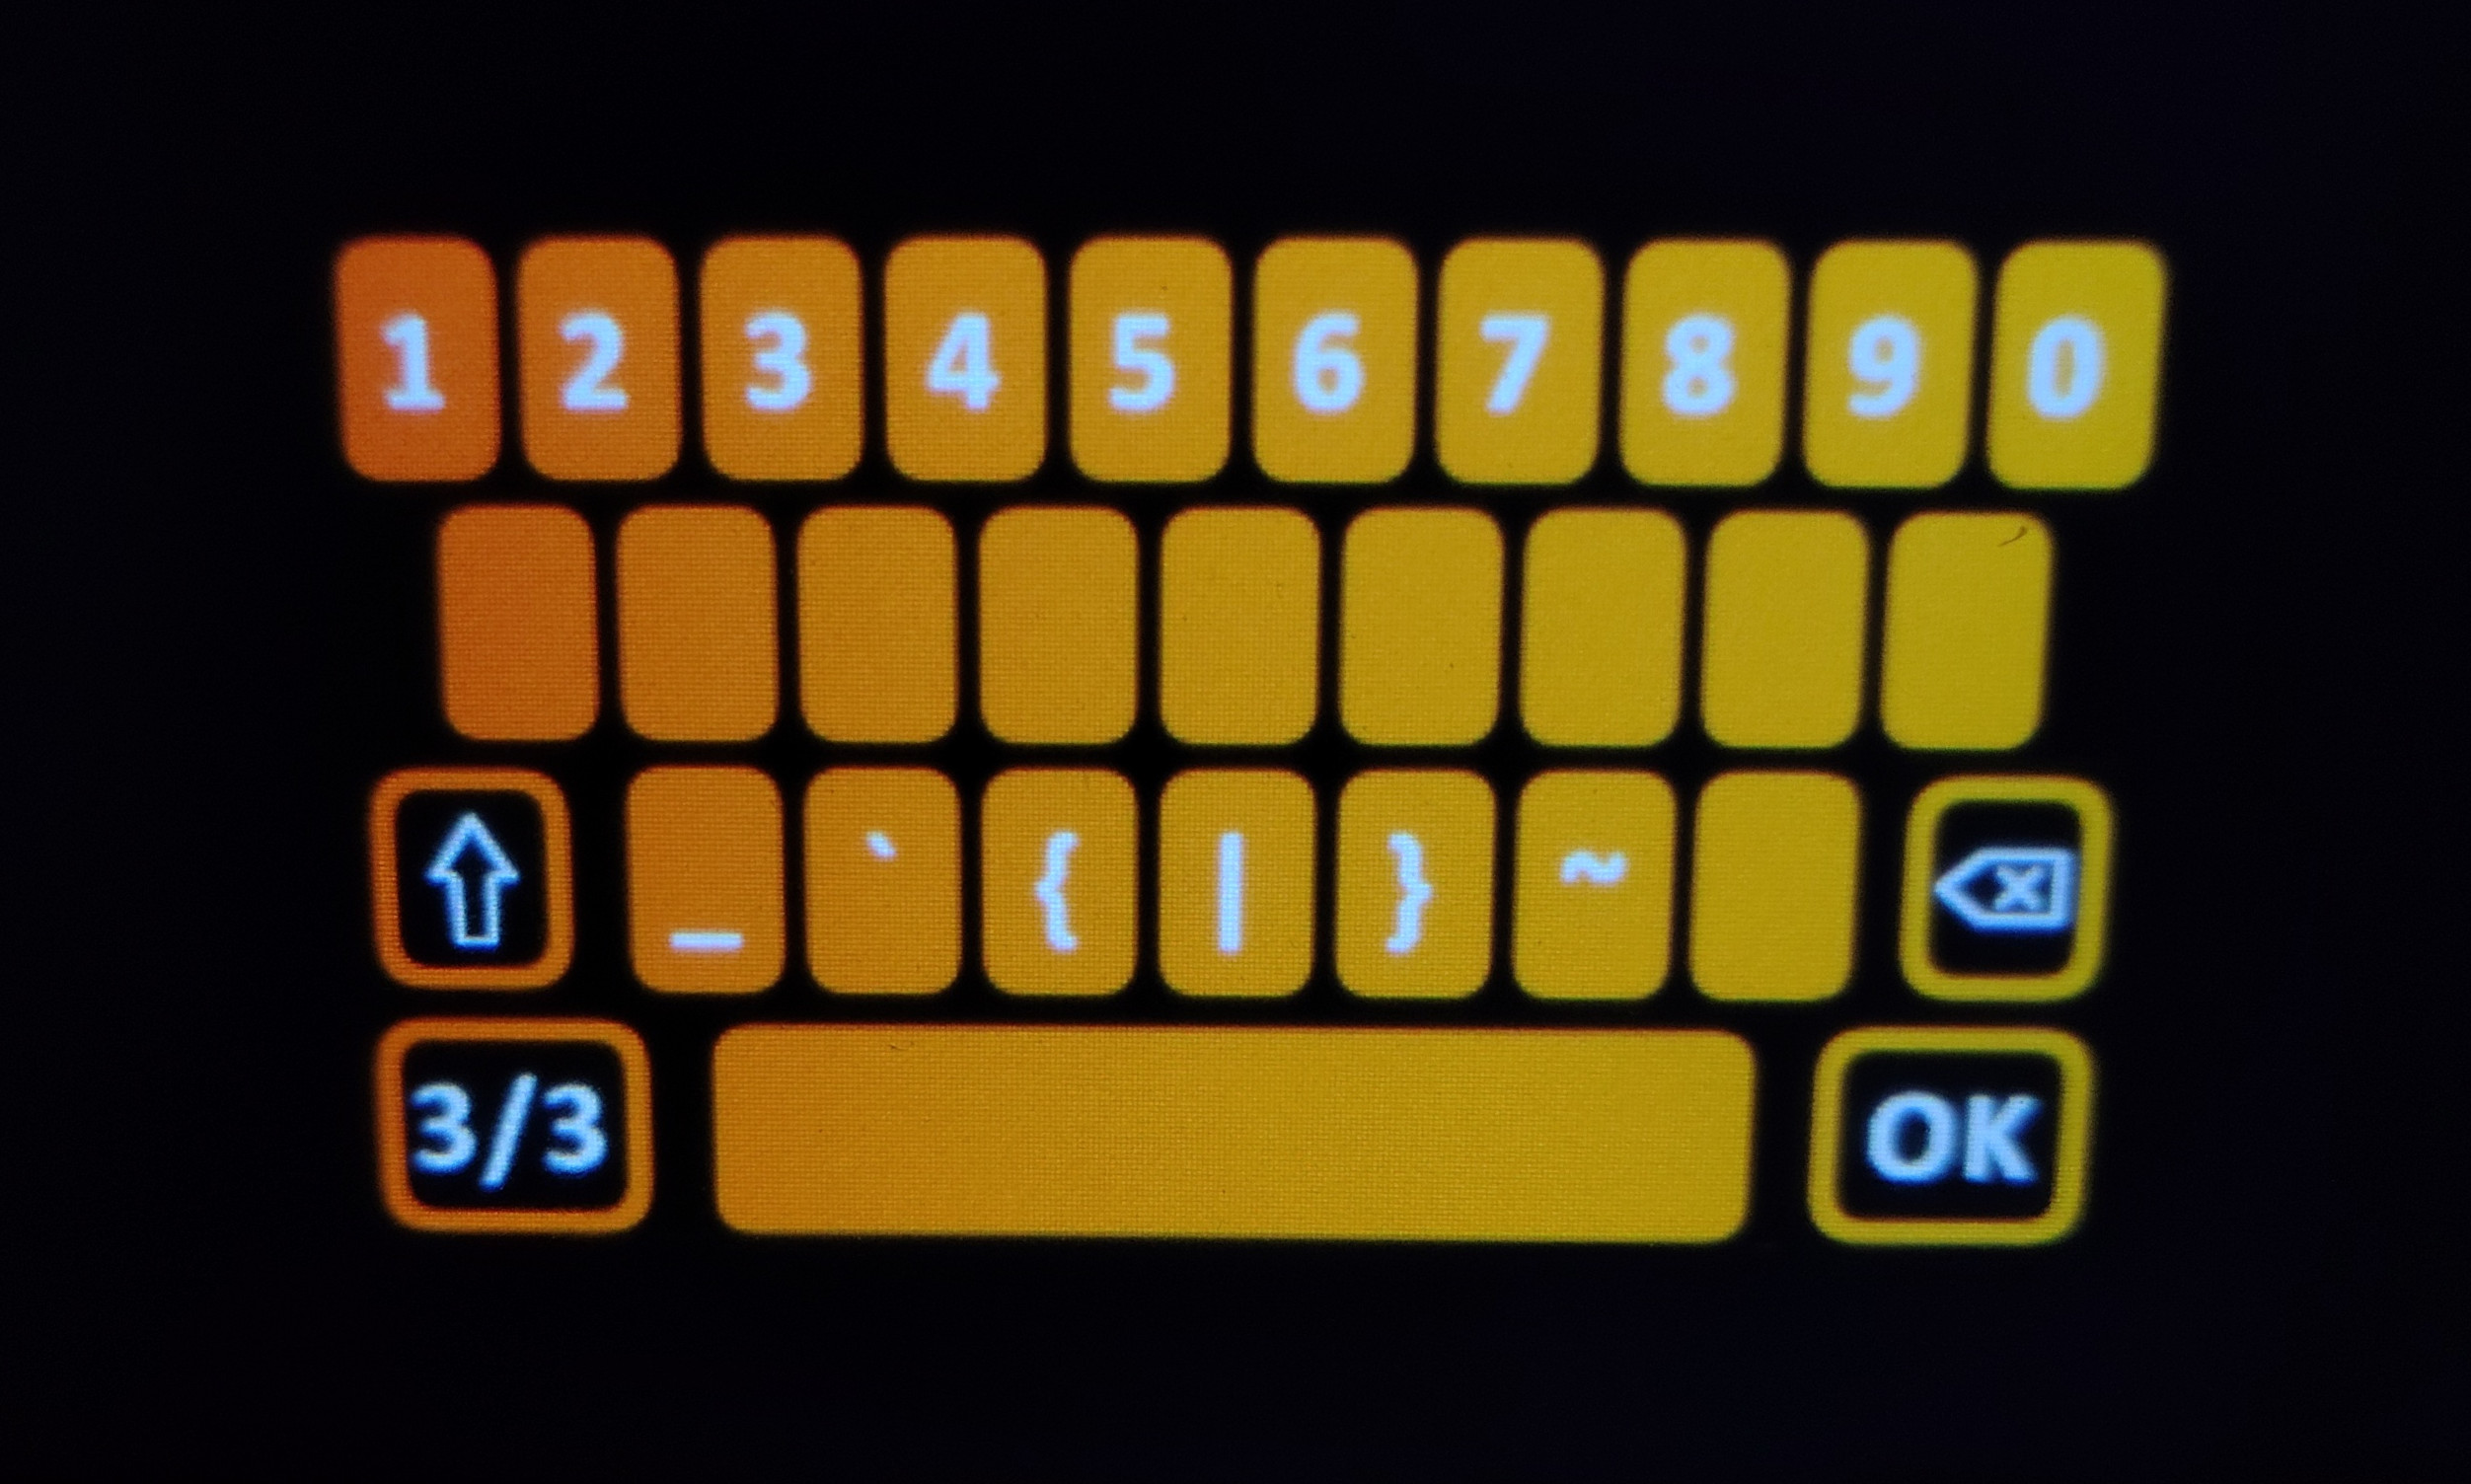
\includegraphics[width=\linewidth]{figures/keyboard_page3.jpg}
        \caption{Third charset: Numbers and more.}
    \end{subfigure}
\end{figure}

The \textbf{second charset} is for symbols and the \textbf{third one} is for numbers and other special characters.
To move to the third charset just press the \textbf{“2/3”} button on the bottom left corner of the keyboard.
When on the third charset, you can switch back to the first charset by pressing the \textbf{“3/3”} button.
In these two pages the shift button won't do anything because it is not needed.\\

When you are done typing, press the \textbf{OK} button to confirm your input and return
to the previous MQTT or WiFi settings page, where the edited field will be updated.

\subsection{The number-only keyboard}

In some fields, such as the MQTT publish frequency, only numbers are allowed.
In this case, ToM+ will open a number-only keyboard page as shown in the image below.

\begin{figure}[H]
    \centering
    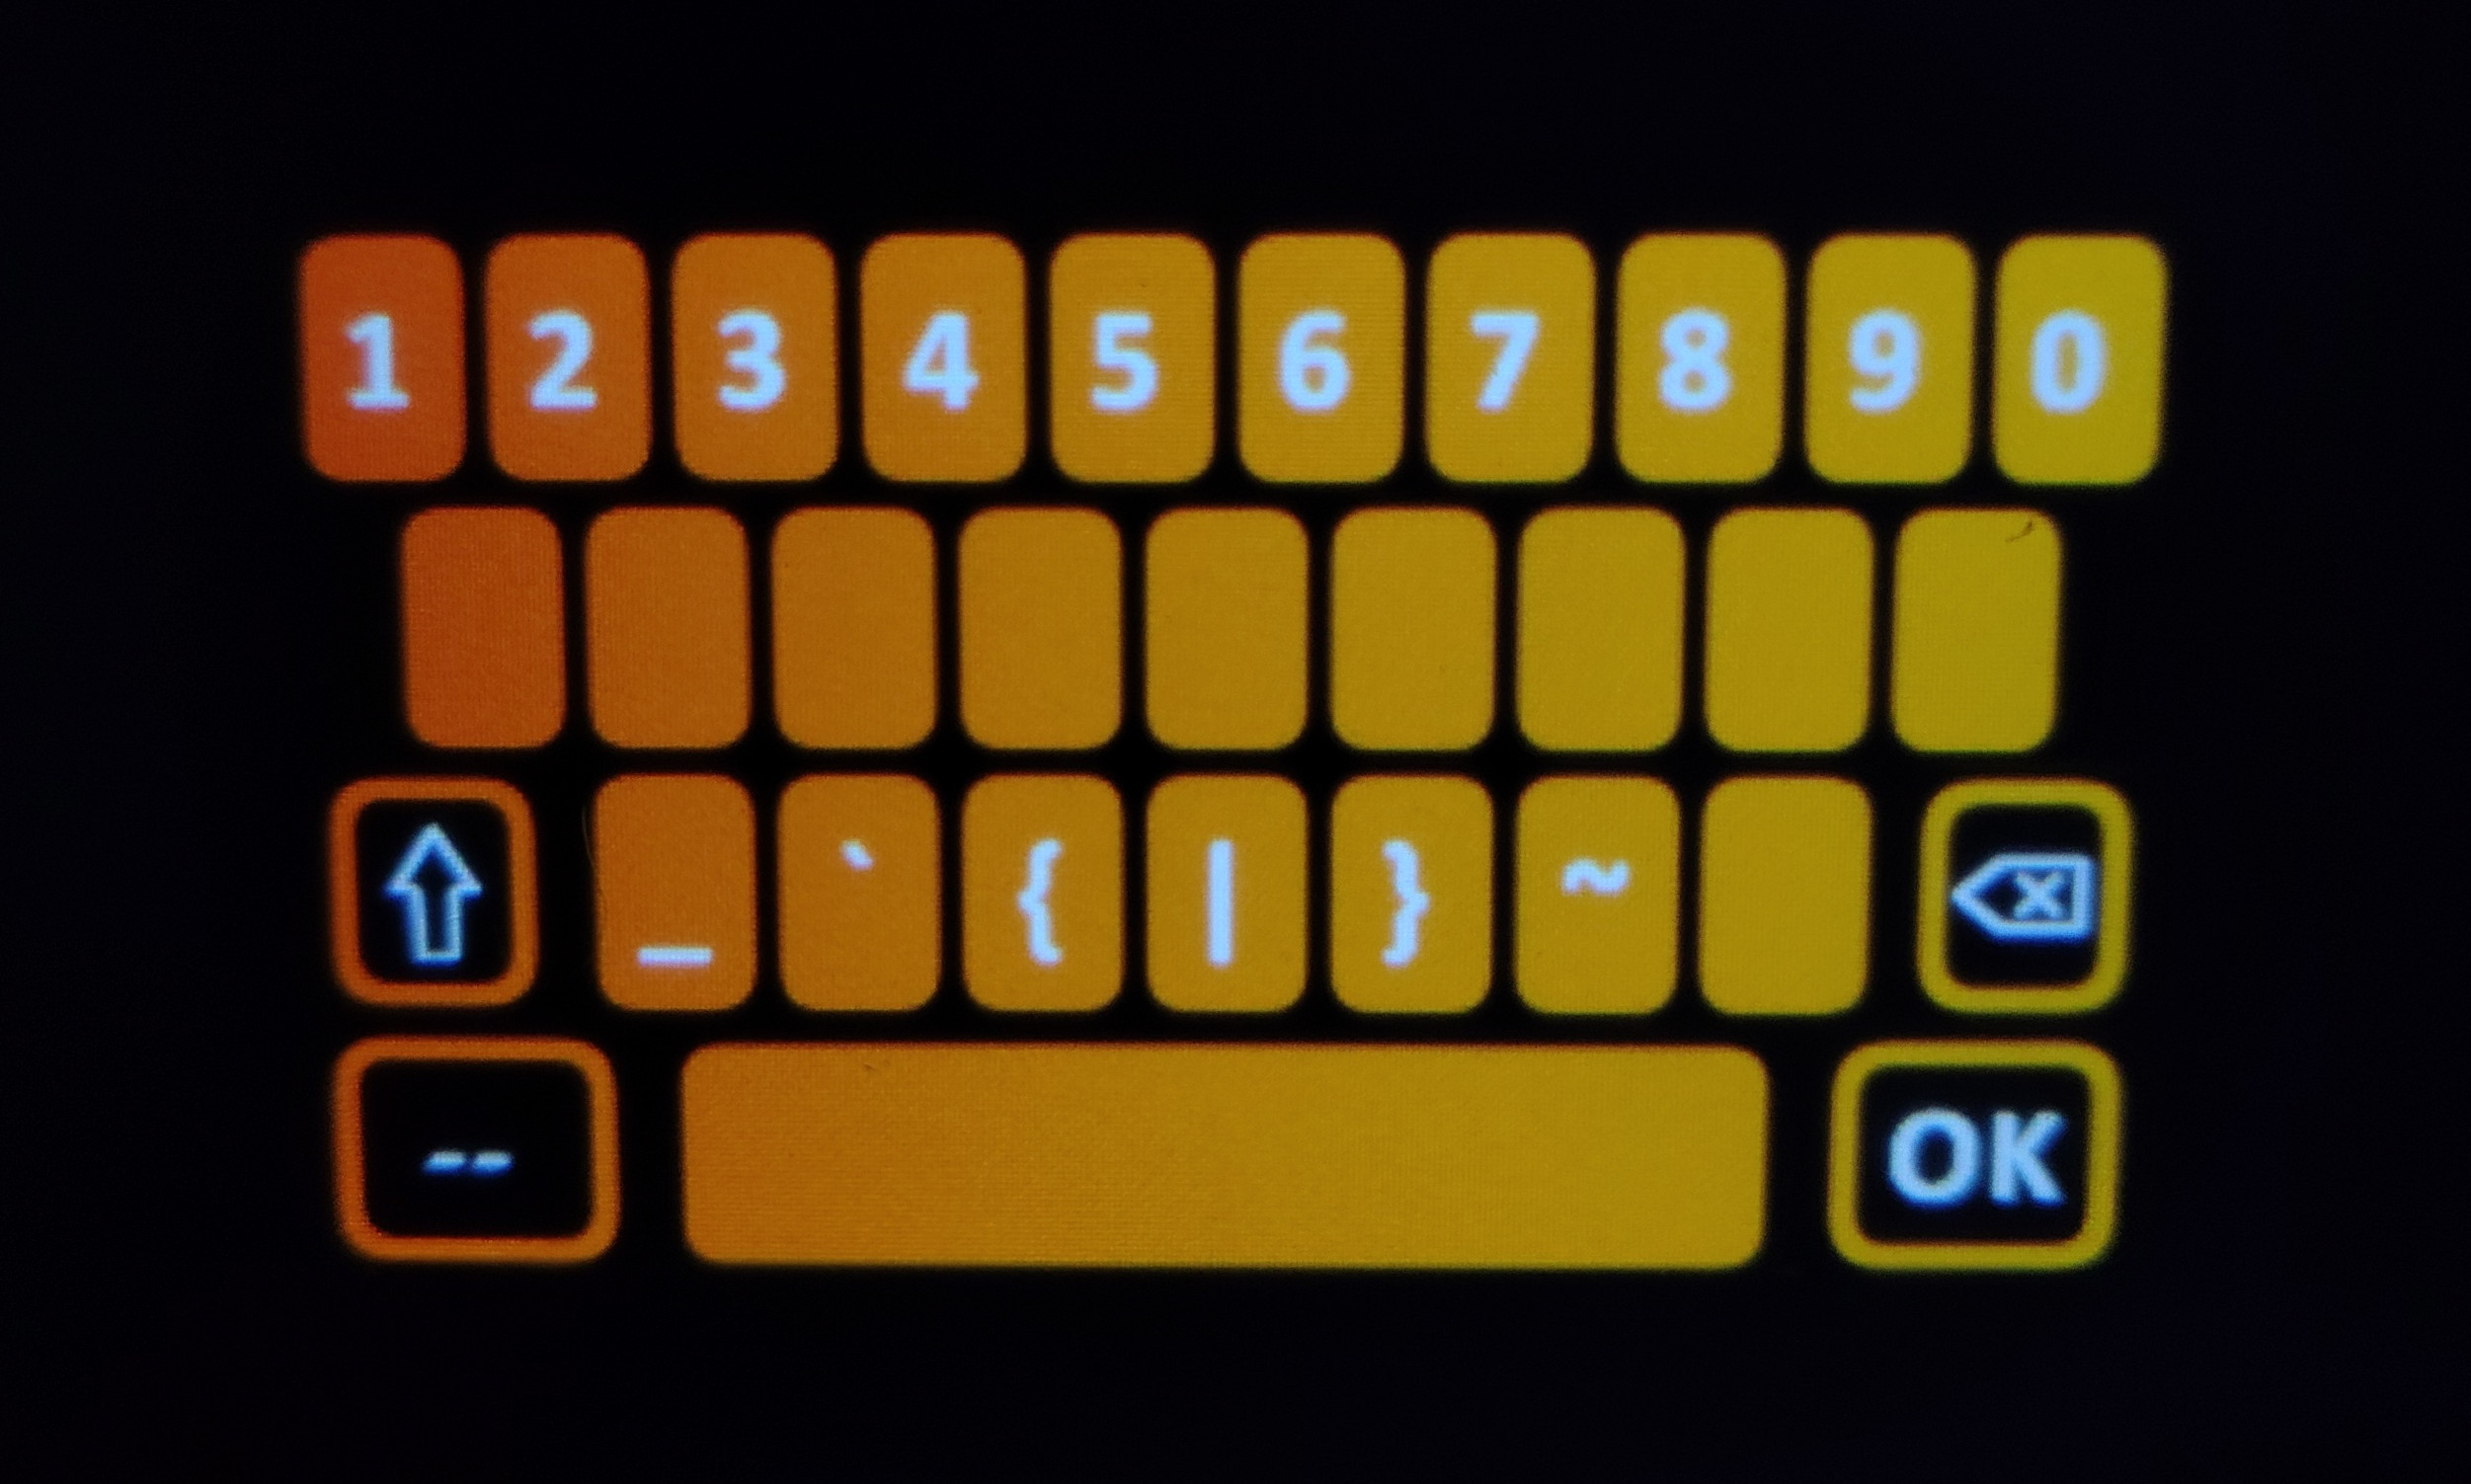
\includegraphics[width=0.8\textwidth]{figures/keyboard_num_only.jpg}
    \caption{Number-only keyboard.}
\end{figure}

As you can see, the layout is the same as the third charset of the full keyboard, but it is limited to numbers and a few special characters.
You can also notice that the change charset button is unavailable, as it is not needed in this case.
The backspace button is still available to delete characters, and the \textbf{OK button} confirms your input and returns to the previous page.



\section{The web server}
\label{sec:web_server}

The web server is a new feature introduced with the second firmware release. 
It allows you to access your ToM+ settings and data remotely from any device with a
web browser, such as your smartphone, tablet, or PC. This is particularly useful 
for managing standard and \textbf{advanced configurations} that aren't available on the ToM+ display.

In addition, you can also use the web server to set up \textbf{WiFi and MQTT} much more easily 
than using the ToM+ display with the keyboard page only (Section~\ref{sec:keyboard_page}).\\

\begin{figure}[H]
    \centering
    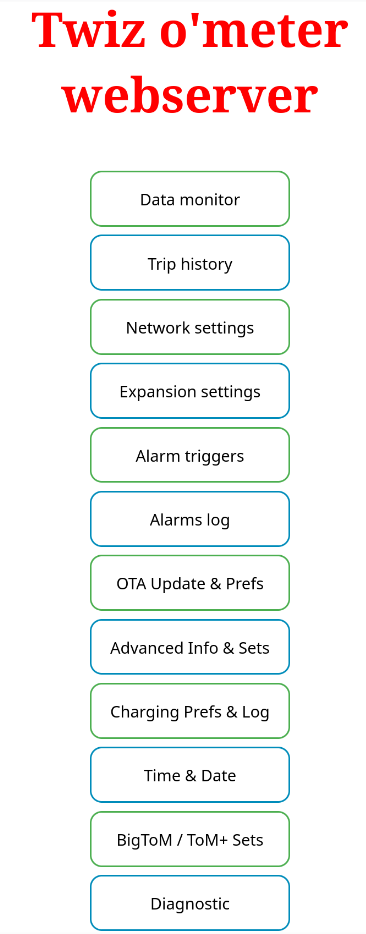
\includegraphics[width=0.46\textwidth]{figures/landing_page.png}
    \caption{Landing page of the web server.}
\end{figure}


\subsection{The landing page}

In the landing page shown above, you will see twelve buttons that give you access to different pages of the web server.
Here I will give a quick overview of the functions available on each page and then in the next paragraphs
they will be all deepen more. In these section, the icons are used as a visual aid only:\\

\iconbox{icons/BatteryInfo2.png}
{Data monitor}{Here you can monitor your Twizy data in real time, organized in tables just like on the ToM+ display pages (Section~\ref{sec:web_data_monitor}).}

\iconbox{icons/Street0Ok_v2.png}
{Trip history}{Here you can check each recorded trip data (1 to 5) and the last twenty trips, the same as on the ToM+ display (Section~\ref{sec:web_trip_history}).}

\iconbox{icons/Tray_WiFiOff.png}
{Network settings}{Here you can set up your Wi-Fi connection profiles and MQTT broker parameters, just like on the ToM+ display (Section~\ref{sec:web_network_settings}).}

\iconbox{icons/Pin1.png}
{Expansion settings}{Here you can configure the expansion connector pins and choose the behavior for the right wiper stalk button (Section~\ref{sec:web_expansion_settings}).}

\iconbox{icons/Alarm.PNG}
{Alarm Triggers}{Here you can view or set up alarms based on ToM+ data and choose the action to be executed when an alarm triggers (Section~\ref{sec:web_alarm_triggers}).}

\iconbox{icons/Alarm.PNG}
{Alarms log}{Here you can view and clear the history of the last 21 alarms trigger and their details, such as date and time (Section~\ref{sec:web_alarms_log}).}

\iconbox{icons/Swap.png}
{OTA Update \& Prefs}{Here you can update the ToM+ firmware via OTA method and backup/restore your ToM+ preferences (Section~\ref{sec:web_ota_update}).}

\iconbox{icons/Swap.png}
{Advanced Info \& Sets}{Here you can view advanced information about your Twizy battery and configure miscellaneous settings (Section~\ref{sec:web_advanced_info}).}

\iconbox{icons/CEta.png}
{Charging Prefs \& Log}{Here you can set up charging preferences, abort charge on the fly, and view or clear the last 15 charging logs (Section~\ref{sec:web_charging_prefs}).}

\iconbox{icons/Timer.PNG}
{Time \& Date}{Here you can set the time and date of your ToM+ and choose the time zone using POSIX TZ strings or synchronize with WiFi (Section~\ref{sec:web_time_date}).}

\iconbox{icons/Kmh.png}
{BigToM \textbackslash ToM+ Sets}{Here you can configure some dashboard parameters, such as the scale of the power bar or setting up a speed limit (Section~\ref{sec:web_btom_tom_sets}).}

\iconbox{icons/Error.png}
{Diagnostic}{Here you can view DTC/DF numbers and the descriptions of your Twizy errors and clear the logs if needed (Section~\ref{sec:web_diagnostic}).}


\subsection{Access the web server}

ToM+ allows you to connect to its web server page in two ways, and they are both
useful in different situations. Before we start, bear in mind that an \textbf{IP address}
it's basically the numeric name of your device on a network (e.g. \textit{192.168.1.100}).

\textbf{\textit{For both methods, you need ToM+ to be connected to a network.}}
So, be sure to check if your ToM+ has either a Wi-Fi profile configured as
explained in Section~\ref{sec:add_wifi_profile} or is connected to a no-password WiFi network.
To check if your ToM+ is connected please refer to Section~\ref{sec:check_wifi_connection}.\\

\textbf{The first and easier setup} is using your phone hotspot without any password, so that ToM+ connects
without having to configure any WiFi profile. Then, still using your phone, go on Chrome or
Safari (or any web browser) and type in ToM+ IP address (shown as Figure~\ref{fig:wifi_bottom_line}).\\

\textbf{The second method} works only when you are quite near to the Twizy within WiFi range.
You can use your phone or laptop to perform a WiFi scan and then search for either
\textit{“ToM+ AP”} or \textit{“Twiz o'Meter AP”} or \textit{“BigToM AP”} network, depending on your model. 
Next, you should connect to that network with the \textbf{correct password}. It is initially 
set to the word “pass” followed by your device serial number (e.g. \textit{pass129777}).
Serial number can be found in the settings page as explained in Figure~\ref{fig:settings_page}. 
Then you can change it if you want, but there's no password recovery system (see Section~\ref{sec:web_change_password}).
Once you are connected to ToM+ Access Point, type on any browser his static IP address, which is \textbf{192.188.1.188}.


\subsection{Change web server password}
\label{sec:web_change_password}

To change the password for the web server, go on the display WiFi settings page (Section~\ref{sec:wifi_settings})
and tap on the \textbf{“KEY 4”} field. This will open the keyboard page (Section~\ref{sec:keyboard_page}) where you can type in your new password.
So, this password will be used for both the Access point password as well as the fourth WiFi connection profile.


\subsection{Data monitor page}
\label{sec:web_data_monitor}

As said in the introduction, this page lists all available ToM+ data, organized into seven
different tables, each of which contains only the data specified in its header. The data
distribution is the same used in Section~\ref{sec:icon_list} and can't be modified.

These values are \textbf{updated every 10 seconds} and are coupled with their measure unit. Don't worry
for your privacy because your data travels packed in a particular packet structure that
is difficult to sniff or crack. In addition, the web server does not use any external
services or MQTT for the monitoring so that your data remains private and safe. The page is fully
generated directly by the black box and doesn't undergo any further processing.

\begin{figure}[H]
    \centering
    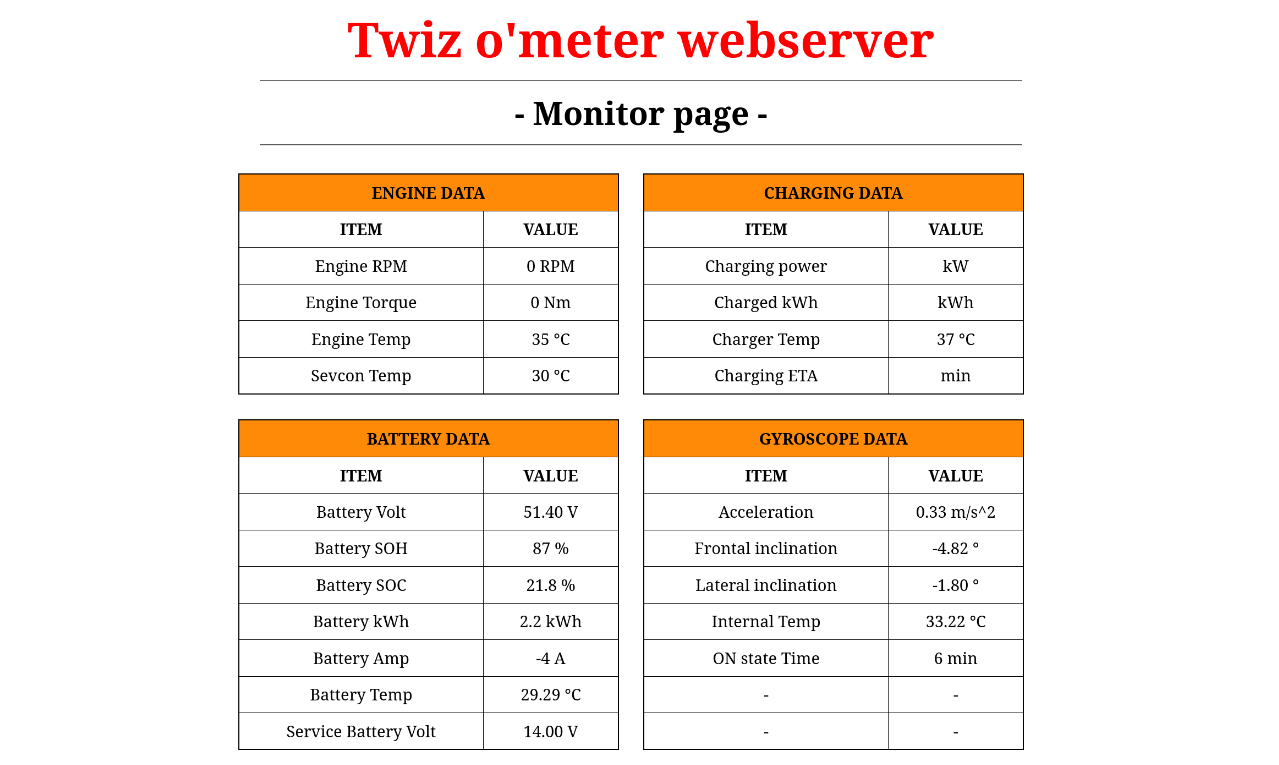
\includegraphics[width=1\textwidth]{figures/monitor_page1.png}
    \caption{Data monitor page (top tables).}
\end{figure}

In the second part of the page, there are the last three tables which contain dashboard data,
expansion port data and the last one holds all the battery info voltages and temperatures.
Press the \textbf{“HOME”} green button pointed by the red arrow to return to the landing page.

\begin{figure}[H]
    \centering
    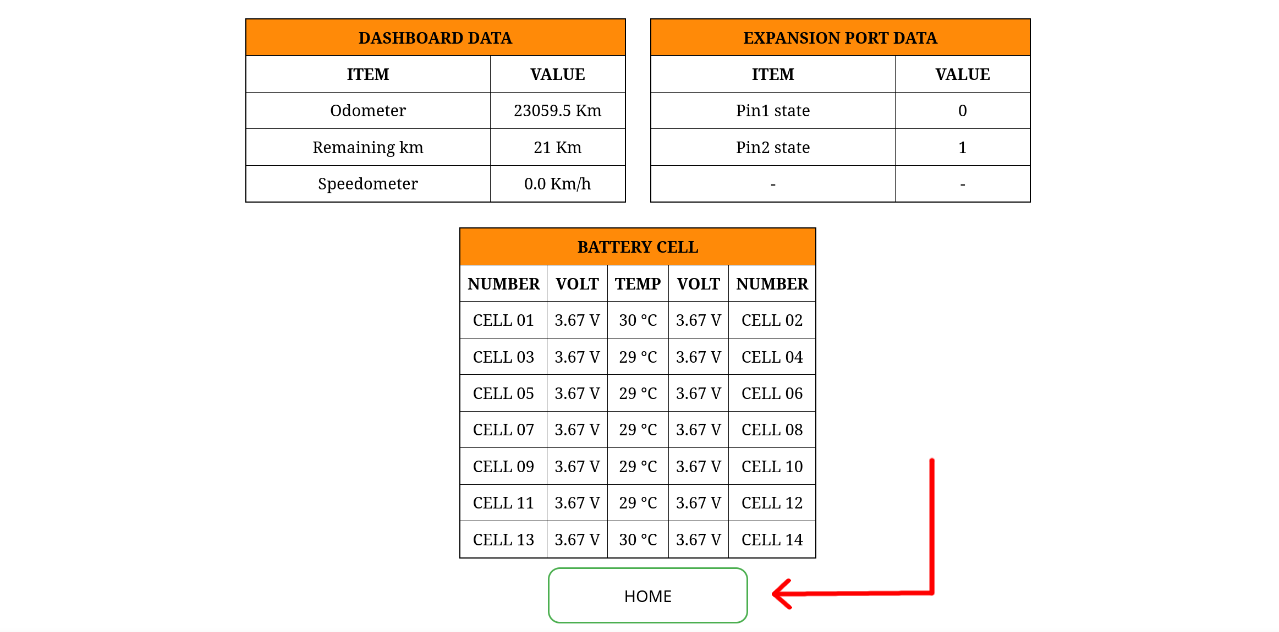
\includegraphics[width=1\textwidth]{figures/monitor_page2.png}
    \caption{Data monitor page (bottom tables).}
\end{figure}

\clearpage

\subsection{Trip history page}
\label{sec:web_trip_history}

This holds the values of the trip page previously discussed in Section~\ref{sec:trip_page}.
It can store up to 5 different sets of data and, even if display shown data are limited,
the web server page will show them all. The first table shows trips, each organized into five rows and
the headers of each record are listed in Section~\ref{sec:icon_list}.

\begin{figure}[H]
    \centering
    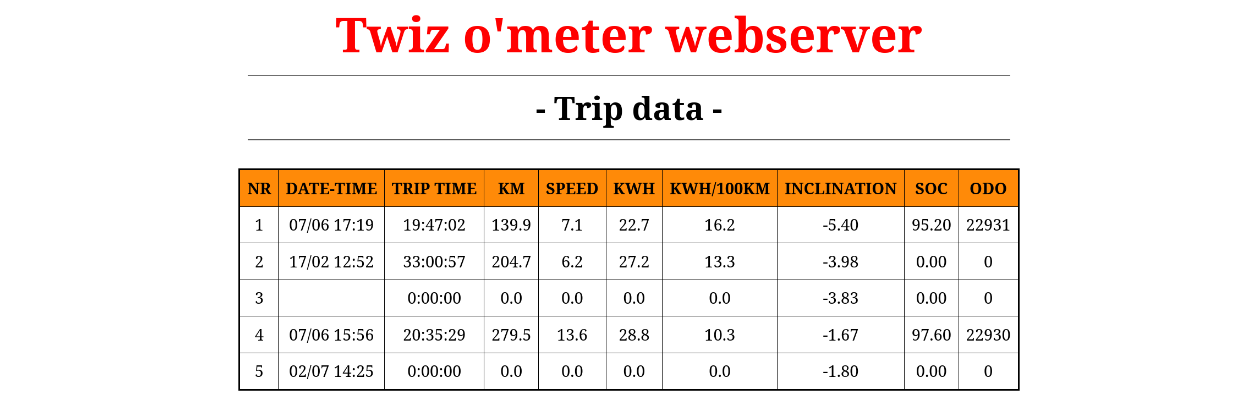
\includegraphics[width=1\textwidth]{figures/trip_page1.png}
    \caption{Trip history page --- Trip data.}
\end{figure}

The second table shows the last twenty trips (from the most recent), with the same headers as the first table.
You can get back to the start page pressing the \textbf{“HOME”} green button located just below the second table.

\begin{figure}[H]
    \centering
    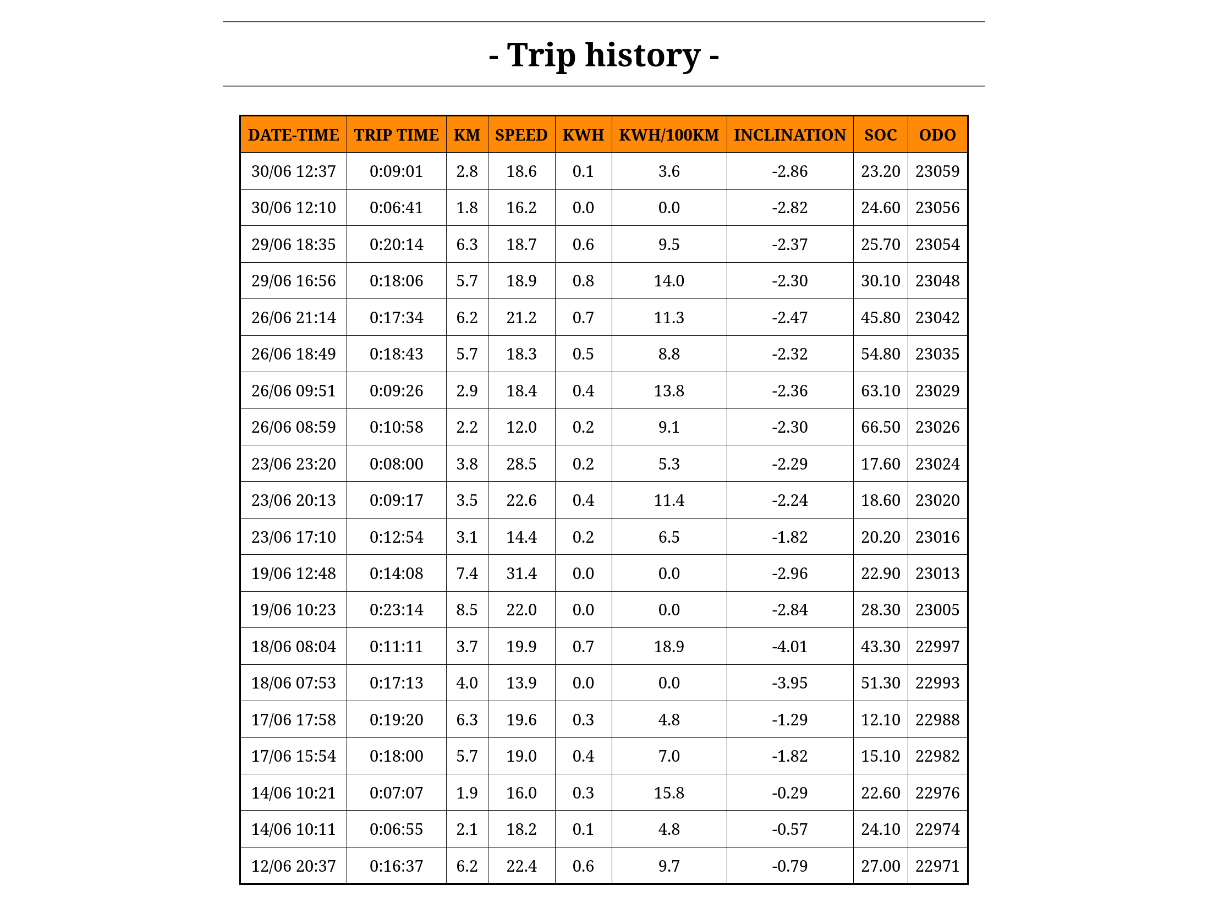
\includegraphics[width=1\textwidth]{figures/trip_page2.png}
    \caption{Trip history page --- Trip history.}
\end{figure}


\subsection{Network settings page}
\label{sec:web_network_settings}

This page allows you to configure Wi-Fi profiles and MQTT broker without struggling with
the ToM+ display keyboard. The page is split in two main tables, one for 
Wi-Fi (Section~\ref{sec:wifi_settings}) and the other for MQTT settings (Section~\ref{sec:MQTT}).\\

As you can see in the image the first one contains all the four profiles that were
previously set on ToM+, or if not, their default values. The same is for passwords, 
that are not visible until you press the “O” button next to the one you want to see. 
Pressing it again will hide the password. 
Here you can also change the Wi-Fi password for the Access Point (Section~\ref{sec:web_change_password}).

\begin{figure}[H]
    \centering
    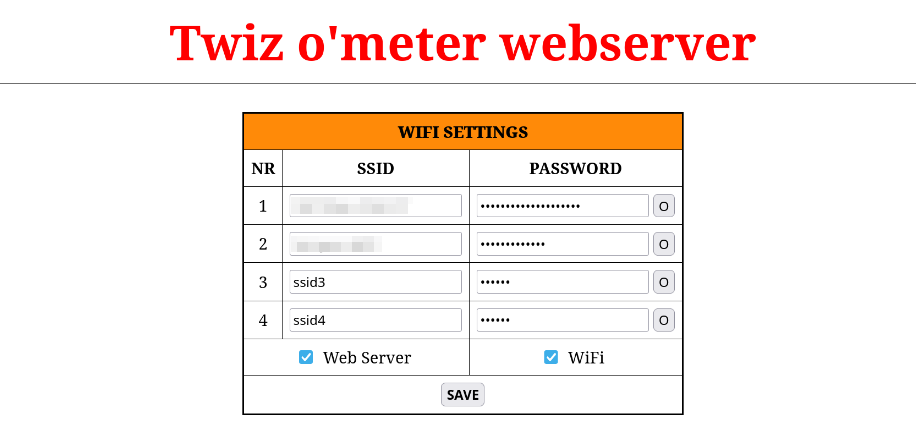
\includegraphics[width=1\textwidth]{figures/wifi_page1.png}
    \caption{Network settings page --- WiFi table.}
\end{figure}

The two check boxes do the same functions as the two sliding buttons in ToM+ WiFi
settings page. To know what they are used for, refer to Section~\ref{sec:enable_disable_wifi}.
After any change, press the \textbf{“SAVE”} button to save your changes, otherwise they will be lost when you leave the page.

\begin{figure}[H]
    \centering
    
\includegraphics[width=1\textwidth]{figures/wifi_page3.png}
    \caption{Network settings page --- WiFi status table.}
\end{figure}

If your ToM+ is connected to a network, a small table will appear below the one just
discussed and the rows contain three main information: the SSID, ToM+ IP address
and the MAC address. These data can be found on the ToM+ display as well, in the
Wi-Fi settings page as previously shown in Figure~\ref{fig:wifi_bottom_line}.\\

The second main table, instead holds the MQTT broker settings, as they were
previously configured on ToM+ display, or if not, default values (\textit{e.g. “broker.address”}).
You can easily change them manually from this web server page, that is much
more comfortable than using the ToM+ display keyboard. Check below in the image
how this table may look once configured.

\begin{figure}[H]
    \centering
    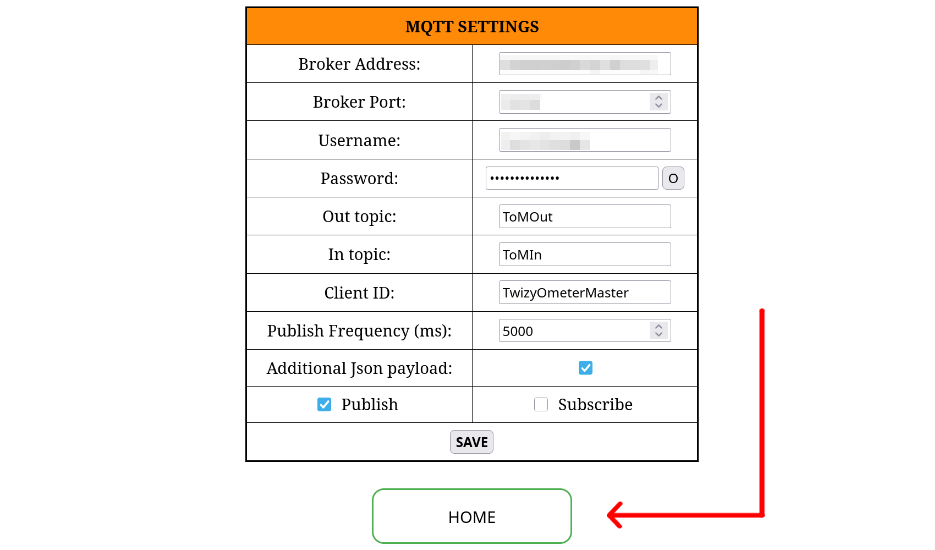
\includegraphics[width=1\textwidth]{figures/wifi_page2.png}
    \caption{Network settings page --- MQTT table.}
\end{figure}

The two check boxes do the same functions as the two sliding buttons in ToM+ MQTT
settings page. To know what they are used for, refer to Section~\ref{sec:enable_disable_mqtt}.
If your ToM+ is connected to the MQTT broker, the table header will have a \textbf{“(CONNECTED!)”} text.\\

After any change, press the \textbf{“SAVE”} button to save your changes, otherwise they will be lost when you leave the page.
At the end of this page, pointed by a red arrow in the image, there's the \textbf{“HOME”} green button to return to the landing page.


\subsection{Expansion settings page}
\label{sec:web_expansion_settings}

This page holds the configuration for PIN1 and PIN2 of the expansion connector, as well as the configuration for the right wiper stalk button.
It can be really useful if you like customizing stuff and adding your personal touch to your ToM+.
The pin-out of the expansion connector is shown in Figure~\ref{fig:expansion_pinout}. 
Since they are general input/output pins you can choose the mode of each one depending on your needs.\\

If you choose the \textbf{“INPUT”} mode, then that line will be listening to the signal specified
in the next field, and this can be really useful when setting a really specific alarm, but
we will discuss this later. On the other hand, if you select the \textbf{“OUTPUT”} mode ToM+
will transmit the signal specified in the next field, which can be HIGH (5V) or LOW
(0V), when an alarm triggers. But as said before, it will be depth in Section~\ref{sec:web_alarm_triggers}.\\

Since the most recent firmware releases, new modes other than INPUT and OUTPUT have been added to the expansion PINs. Let's dig into them:\\

\begin{itemize}
    \item \textbf{IR CONTROLLER}: This mode allows ToM+ to be controlled by an infrared remote.
    \item \textbf{KEY+ CONTROLLER}: This mode allows you to control your ToM+ via a rotational infrared remote. For these two first modes an additional configuration table will appear.
    \item \textbf{SERIAL TX}: Allows you to configure a serial TX line (still not implemented).
    \item \textbf{SERIAL RX}: Allows you to configure a serial RX line (still not implemented).
    \item \textbf{CTRL BUTTON}: This mode allows you to use the right wiper stalk button as a control button for your ToM+ gestures.
\end{itemize}

\subsubsection{Standard OUTPUT mode}

Both in \textbf{“OUTPUT”} and \textbf{“INPUT”} mode, you will need first of all to choose between
\textit{“Active High”} or \textit{“Active Low”}. When an alarm triggers a LOW/HIGH signal is sent
to the PIN chosen as the alarm output (either PIN1 or PIN2).

If you select \textit{“Active High”}, the signal sent is HIGH (5V) and normally is held to LOW (0V).

If you select \textit{“Active Low”}, the signal sent is LOW (0V) and normally is held to HIGH (5V).

\begin{figure}[H]
    \centering
    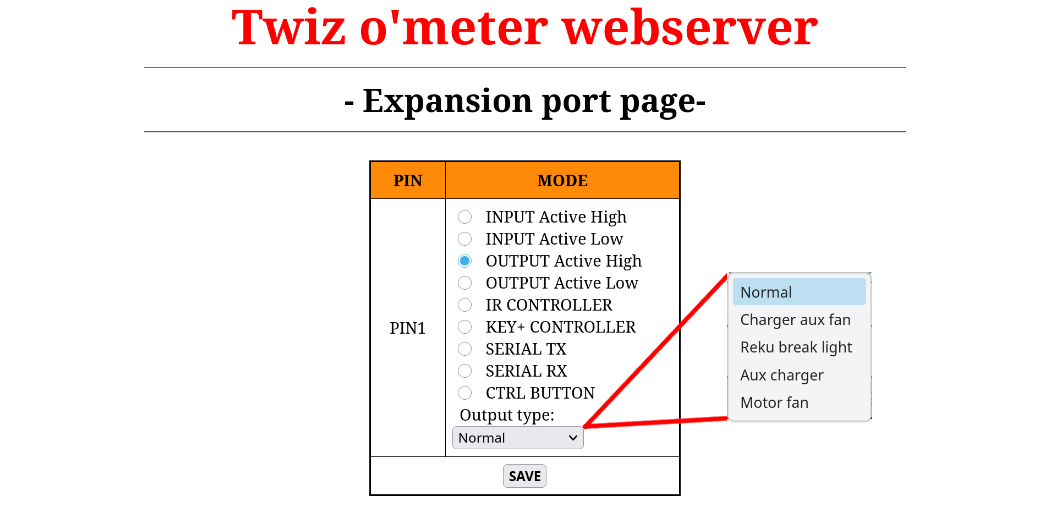
\includegraphics[width=1\textwidth]{figures/expansion_page1.png}
    \caption{Expansion settings page --- PIN1 table.}
\end{figure}

As you can see in the image below, when selecting the \textbf{“OUTPUT”} mode, you can also choose
the \textit{“Output Type”}. This is useful if you have a really specific output device that
needs additional management that is not limited to the standard HIGH/LOW signal. To achieve this,
you can choose from a list of already managed output devices, highlighted in the image above.\\

After any change, press the \textbf{“SAVE”} button to save your changes, otherwise they will be lost when you leave the page.
If you got an idea for a new output device that can be useful for the community, feel free to contact me.\\

\begin{itemize}
    \item \textit{“Normal”}: This is the standard OUTPUT mode, limited to HIGH/LOW signals.
    \item \textit{“Charger auxilliary fan”}: This lets you control an auxilliary fan. 
    You will need to set an alarm on charger temperature with a threshold. Then, when charging, if 
    it triggers the fan will start cooling the charger, stopping only after the temperature
    drops below the selected threshold with a fixed hysteresis (even after charging is finished if needed).
    \item \textit{“Reku break light”}: This lets you connect a relay board which controls
    the breaking light, in order to power it on when in regeneration mode. This is particularly
    useful if your Twizy is tuned to increase the regeneration power.
    \item \textit{“Auxilliary charger”}: This lets you control an auxilliary charger with an
    alarm on SOC or battery voltage. It lets you connect a relay board that enables or disables an
    auxilliary charger when needed. It powers on only in charging mode, with a small fixed delay.
    \item \textit{“Motor fan”}: This lets you control a motor fan with an alarm on the engine temperature.
    It works the same as the charger fan with the difference that this works only while driving.
\end{itemize}

\subsubsection{Standard INPUT mode}

As you can see in the image below, when selecting the \textbf{“INPUT”} mode, no additional tables will appear.
This mode heavily relies on alarm configuration and triggers, so plese refer to Section~\ref{sec:web_alarm_triggers}.
We chose \textbf{“INPUT”} mode in the second table, that works the same but it's intended for PIN2 of the expansion connector.

After any change, press the \textbf{“SAVE”} button to save your changes, otherwise they will be lost when you leave the page.

\begin{figure}[H]
    \centering
    
\includegraphics[width=1\textwidth]{figures/expansion_page3.png}
    \caption{Expansion settings page --- PIN2 table.}
\end{figure}

\subsubsection{IR CONTROLLER mode}

First of all you will need an IR receiver (either a sensor or a module like the one in the first image)
to be plugged in one of the expansion board PINs.
This mode is intended to be used with a general IR remote, but the one I personally suggest
is the one shown in the second image below, specially designed to be put on the steering wheel.

\begin{figure}[ht]
    \centering

    \begin{subfigure}[t]{0.48\textwidth}
        \centering
        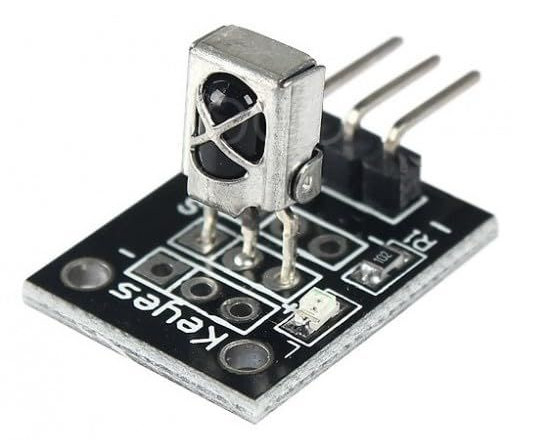
\includegraphics[width=\linewidth]{figures/ir_receiver.jpg}
        \caption{IR receiver module.}
    \end{subfigure}
    \hfill
    \begin{subfigure}[t]{0.48\textwidth}
        \centering
        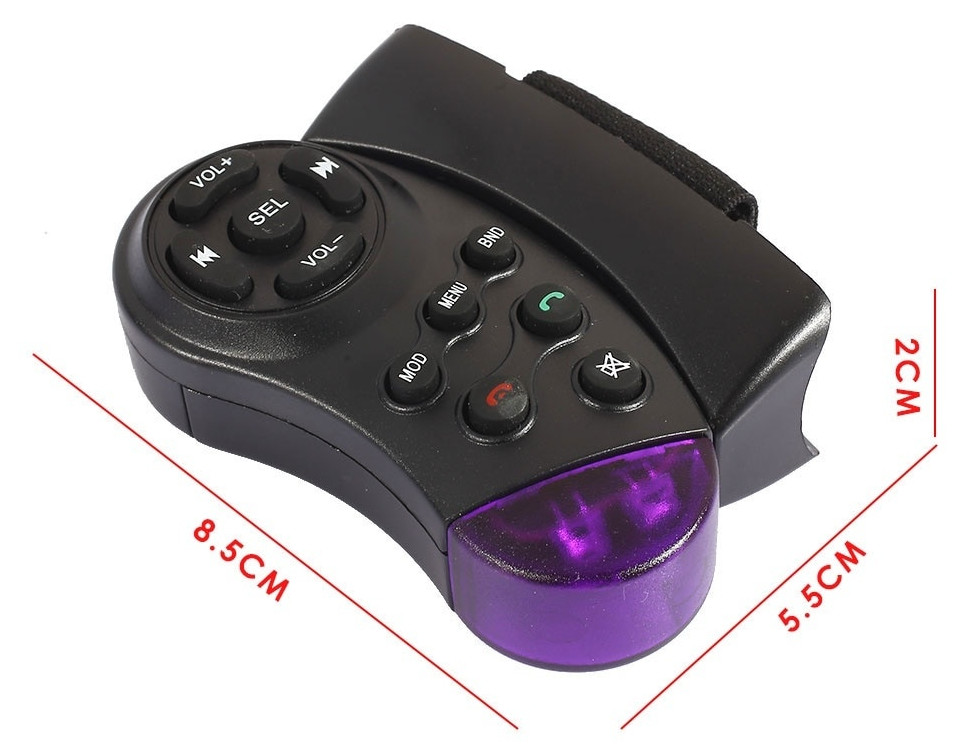
\includegraphics[width=\linewidth]{figures/ir_controller_photo.jpg}
        \caption{IR controller steering wheel remote.}
    \end{subfigure}
\end{figure}

When you select the \textbf{“IR CONTROLLER”} mode for either PIN1 or PIN2 table, remember
to press the \textbf{“SAVE”} button to save your changes. Once you saved, the page will
reload and an additional table will appear below, you can see it in the image below.

\begin{figure}[H]
    \centering
    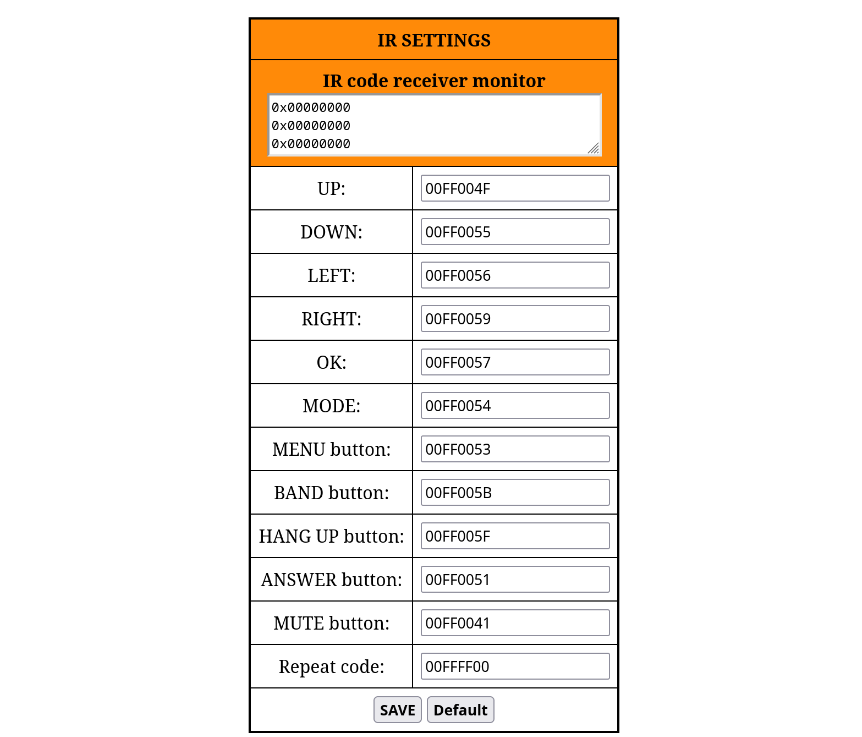
\includegraphics[width=0.8\textwidth]{figures/ir_settings.png}
    \caption{Expansion settings page --- IR settings table.}
\end{figure}

This table will help you to pair each button of the IR controller with the respective IR code.
In the top part of the table there is a little text area that you can use as an \textbf{IR code
receiver moditor} to test in real-time IR codes of your remote after plugging the IR receiver.\\

Using this, you can fill the other fields accordingly. The last one is particularly important
and it's basically the code the remote sends when you are holding down a button.
After that, remeber to press the \textbf{“SAVE”} button to save your changes, otherwise they will be lost when you leave the page.
Lastly, a useful \textbf{“Default”} button is located next to it, to easily revert your changes if needed.

\subsubsection{KEY+ CONTROLLER mode}

This mode is really similar to the one just discussed, but is intended to be used with
another type of controller (the one in the picture below). It's a Bluetooth 
wireless rotary controller for car audio systems, which performs different
actions depending on how fast/slow you are rotating the external ring. And of course it
has some more buttons as well in the internal part.\\

\begin{figure}[H]
    \centering
    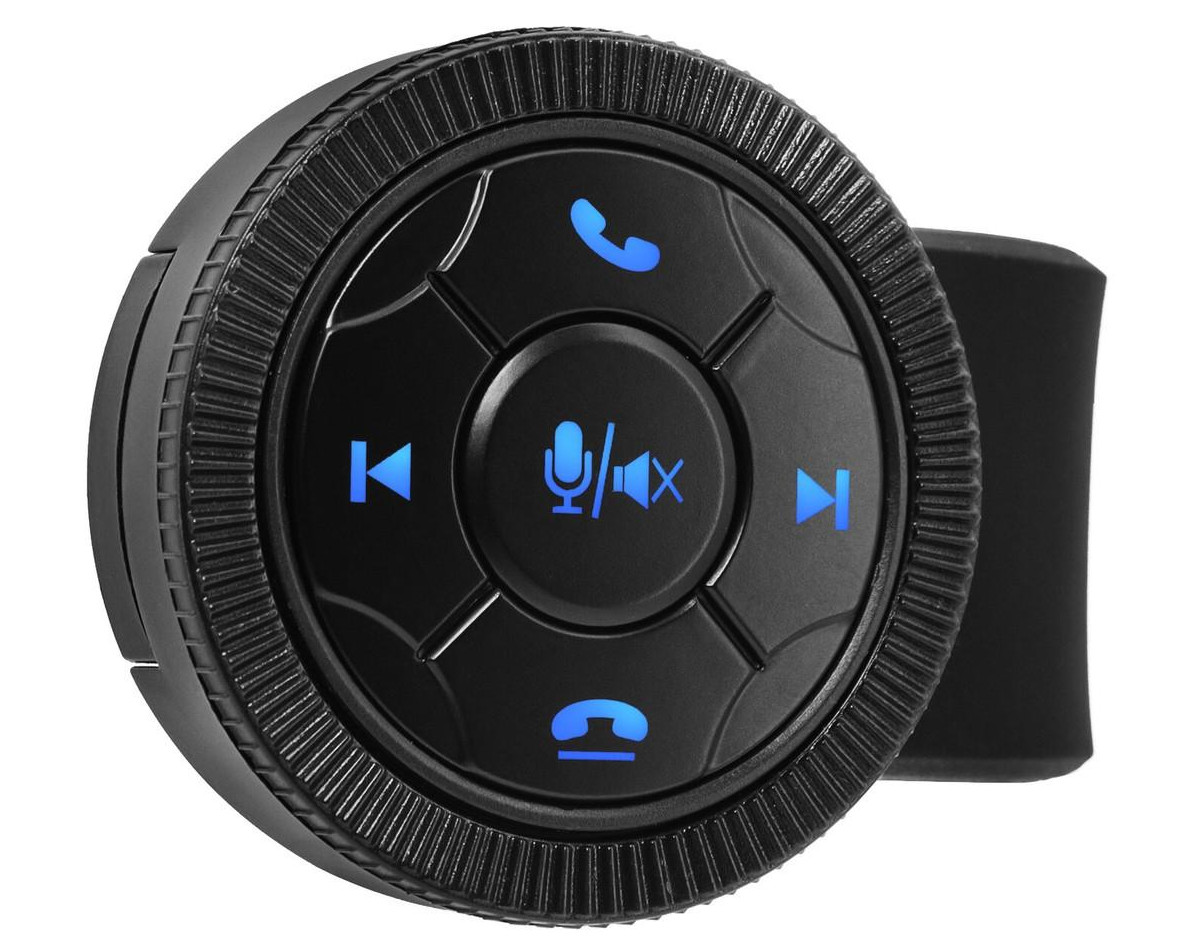
\includegraphics[width=0.4\textwidth]{figures/keyp_controller.jpg}
    \caption{Bluetooth wireless rotary controller.}
\end{figure}

When you select the \textbf{“KEY+ CONTROLLER”} mode for either PIN1 or PIN2 table, remember
to press the \textbf{“SAVE”} button to save your changes. Once you saved, the page will
reload and an additional table will appear below, you can see it in the image below.

\begin{figure}[H]
    \centering
    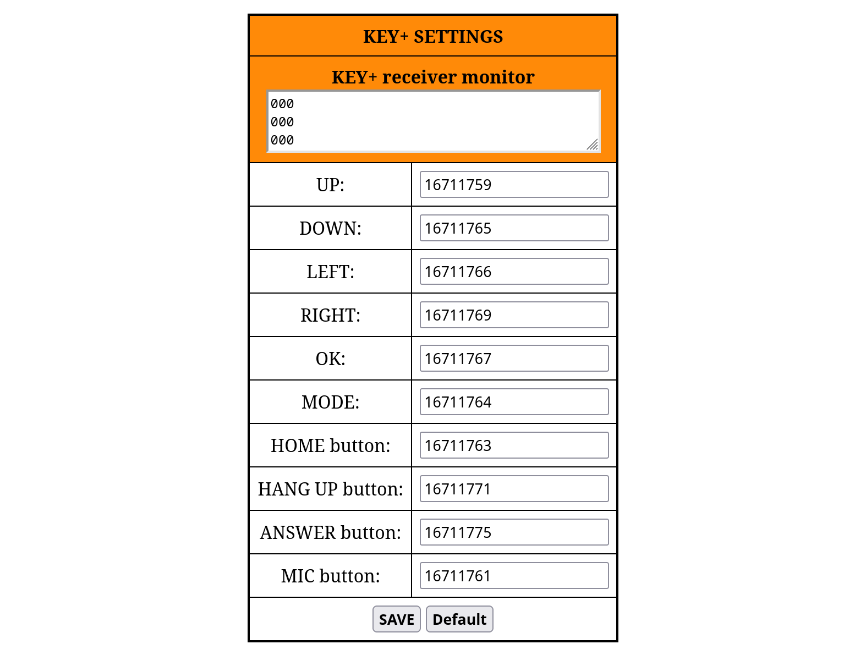
\includegraphics[width=0.8\textwidth]{figures/keyp_settings.png}
    \caption{Expansion settings page --- KEY+ settings table.}
\end{figure}

This works the same as the IR settings table. The main difference is about how ToM+ reads
this values from the expansion port. \todo{TODO}

\subsubsection{CTRL BUTTON mode}

This last table holds the configuration needed to make the provided right \textbf{wiper stalk button} (Figure~\ref{fig:wiper_stalk_button}) work.
You can use this button to navigate through all ToM+ UI without using the touch-screen, with
these three main \textbf{actions}: \textit{“Browse items”}, \textit{“Change page”}, \textit{“Select-deselect”}.
To achieve this, there are three type of \textbf{button presses}: \textit{“Short”}, \textit{“Medium”}, \textit{“Long”}.\\

\begin{figure}[H]
    \centering
    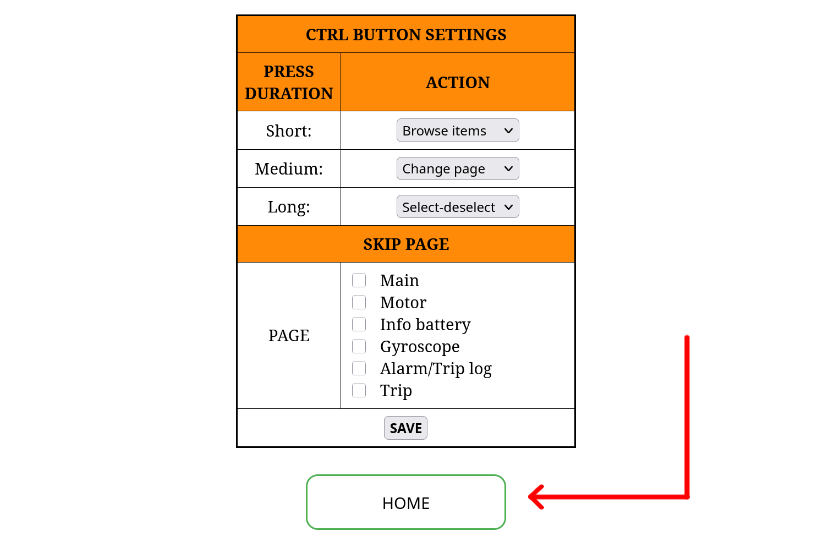
\includegraphics[width=1\textwidth]{figures/expansion_page2.png}
    \caption{Expansion settings page --- Wiper stalk button table.}
\end{figure}

So, in the first part of this table you can rearrange this actions with the gestures you prefer.\\

\begin{itemize}
    \item \textit{“Browse items”}: This moves a small white marker next to the current selected data.
    \item \textit{“Change page”}: This lets you cycle through the pages present in the rotation.
    \item \textit{“Select-deselect”}: This simulates tapping on the selected data (e.g. switches from background to foreground).\\
\end{itemize}

In the second part of the table you can select the \textbf{pages you would like to skip} when
cycling through the available pages repeating the \textit{“Change page”} gesture. For instance,
if I don't want to monitor the Info battery page when cycling with the button, I just check
it out and it will be removed from the rotation.\\

After any change, press the \textbf{“SAVE”} button to save your changes, otherwise they will be lost when you leave the page.
At the end of this page, pointed by a red arrow in the image, there's the \textbf{“HOME”} green button to return to the landing page.

\clearpage

\subsection{Alarm triggers page}
\label{sec:web_alarm_triggers}

